\chapter{Eksperymenty i wyniki}

W tym rozdziale przedstawiono eksperymenty przeprowadzone dla różnych algorytmów na grafach syntetycznych i rzeczywistych. Wszystkie testy były uruchamiane automatycznie za pomocą skryptów z folderu \texttt{src/glopt/cli/}. Wyniki zostały zebrane w plikach CSV i przeanalizowane za pomocą skryptu \texttt{scripts/analyze.py}.

Eksperymenty miały na celu odpowiedzenie na kilka kluczowych pytań:
\begin{itemize}
  \item Które algorytmy dają najlepsze wyniki dla różnych typów grafów?
  \item Jak czas działania algorytmów zmienia się wraz z rozmiarem grafu?
  \item Jakie konfiguracje licencji są najbardziej opłacalne w różnych sytuacjach?
  \item Czy istnieje dobry kompromis między jakością rozwiązania a czasem obliczeń?
\end{itemize}

Rozdział zawiera opis środowiska testowego, parametrów eksperymentów oraz analizę otrzymanych wyników z wykresami i interpretacją.

\section{Środowisko testowe}

\subsection{Konfiguracja sprzętowa i programowa}

Wszystkie eksperymenty zostały przeprowadzone w następującym środowisku:

\begin{itemize}
  \item \textbf{System}: Ubuntu 24.04 LTS na WSL2
  \item \textbf{Procesor}: Intel Core i5-14600KF (16 wątków)
  \item \textbf{Pamięć RAM}: 24 GiB dostępne dla WSL2
  \item \textbf{Python}: wersja 3.13 (wymuszona w projekcie)
  \item \textbf{Główne biblioteki}:
  \begin{itemize}
    \item \texttt{networkx} -- tworzenie i analiza grafów
    \item \texttt{pulp} z solverem CBC -- programowanie liniowe całkowitoliczbowe
    \item \texttt{numpy}, \texttt{pandas} -- obliczenia numeryczne i przetwarzanie danych
    \item \texttt{matplotlib} -- wizualizacje i wykresy
  \end{itemize}
\end{itemize}

\subsection{Metryki i kryteria oceny}

Każdy eksperyment zapisuje do pliku CSV następujące metryki:

\begin{itemize}
    \item \textbf{total\_cost} -- całkowity koszt rozwiązania (suma kosztów wszystkich grup)
    \item \textbf{cost\_per\_node} -- koszt przypadający na jeden wierzchołek (pozwala porównywać grafy różnych rozmiarów)
    \item \textbf{time\_ms} -- czas wykonania algorytmu w milisekundach
    \item \textbf{valid} -- czy rozwiązanie jest poprawne (wszystkie wierzchołki pokryte, ograniczenia spełnione)
    \item \textbf{groups} -- liczba utworzonych grup licencyjnych
    \item \textbf{group\_size\_mean/median/p90} -- statystyki rozmiarów grup
    \item \textbf{license\_counts\_json} -- jakie typy licencji zostały użyte
\end{itemize}

Algorytm ILP (programowanie całkowitoliczbowe) służy jako punkt odniesienia -- daje optymalne rozwiązania dla małych grafów. Pozostałe algorytmy oceniamy porównując ich wyniki do ILP oraz analizując kompromis między jakością a czasem działania.

\section{Rodzaje grafów i konfiguracje licencji}

\subsection{Grafy syntetyczne}

W eksperymentach wykorzystano trzy rodziny grafów syntetycznych:

\begin{itemize}
  \item \textbf{Grafy losowe (random)} -- generowane modelem Erdős–Rényi z prawdopodobieństwem krawędzi $p = 0.10$
  \item \textbf{Grafy małoświatowe (small-world)} -- generowane modelem Watts–Strogatz z $k = 6$ sąsiadów i prawdopodobieństwem przepinania $p = 0.05$
  \item \textbf{Grafy bezskalowe (scale-free)} -- generowane modelem Barabási–Albert z parametrem $m = 2$
\end{itemize}

Każdy typ grafu testuje się dla rozmiarów od 20 do 3000 wierzchołków. Dla każdego rozmiaru generowane są 3 różne grafy, a każdy graf jest testowany 2 razy z różnymi ziarnami losowymi. Daje to łącznie 6 wyników na każdy punkt na wykresie.

\subsection{Grafy rzeczywiste}

W badaniach wykorzystano rzeczywiste sieci społecznościowe z dataset-u Facebook ego-networks (Stanford SNAP). Są to sieci znajomości użytkowników Facebooka. Dataset zawiera 10 różnych sieci o rozmiarach od kilkudziesięciu do kilkuset wierzchołków.

\subsection{Konfiguracje licencji}

W eksperymentach wykorzystano dwie podstawowe konfiguracje licencji, zgodne z definicjami w \texttt{src/glopt/license\_config.py} (szczegóły w aneksie):

\begin{itemize}
  \item \textbf{duolingo\_super} — \emph{Individual} (pojemność 1) oraz \emph{Family} (pojemność 2–6).
  \item \textbf{roman\_domination} — \emph{Solo} (pojemność 1) i \emph{Group} (pojemność \(\ge\)2), z cenami względnymi (por. rozdz.\,\ref{chap:extensions}).
\end{itemize}

W rozszerzeniach (rozdz.\,\ref{chap:extensions}) analizowano również konfigurację \texttt{spotify} oraz warianty cenowe \texttt{roman\_p\_x}.

\section{Parametry eksperymentów}

\subsection{Testowane algorytmy}

W eksperymentach wykorzystano następujące algorytmy (przy pierwszym użyciu podano polską nazwę i angielski odpowiednik; dalej stosujemy nazwy polskie):

\begin{itemize}
  \item \textbf{Programowanie całkowitoliczbowe (ILP)} — solver CBC, limit czasu 60 s
  \item \textbf{Algorytm zachłanny (Greedy)} — deterministyczna heurystyka konstrukcyjna
  \item \textbf{Algorytm losowy (Randomized)} — losowy przydział zgodny z pojemnościami, z fallbackiem na zachłanny
  \item \textbf{Heurystyka zbioru dominującego (Dominating Set)} — konstrukcja przez wierzchołki dominujące
  \item \textbf{Algorytm genetyczny (Genetic Algorithm)} — populacja=30, generacje=40, elita=20\%, crossover=0.6
  \item \textbf{Symulowane wyżarzanie (Simulated Annealing)} — parametry chłodzenia dobrane eksperymentalnie
  \item \textbf{Przeszukiwanie tabu (Tabu Search)} — \emph{tabu tenure}=20
  \item \textbf{Algorytm mrówkowy (Ant Colony Optimization)} — $\alpha=1$, $\beta=2$, parowanie=0.5, $q_0=0.9$, 20 mrówek
\end{itemize}

\subsection{Organizacja eksperymentów}

Eksperymenty uruchamiano za pomocą skryptów:
\begin{itemize}
  \item \texttt{benchmark.py} -- testy na grafach syntetycznych
  \item \texttt{benchmark\_real.py} -- testy na grafach rzeczywistych
  \item \texttt{dynamic.py} -- symulacje dynamicznych zmian w grafie
\end{itemize}

Każdy algorytm ma limit czasu 60 sekund na jedną próbę. Jeśli algorytm nie skończy w tym czasie, jest zabijany i wynik oznaczany jako timeout.

Dla każdego zestawu (typ grafu × rozmiar × konfiguracja licencji) wygenerowano 3 różne grafy i każdy z nich przetestowano 2 razy. Daje to łącznie 6 pomiarów na punkt, co pozwala obliczyć średnie i ocenić stabilność wyników.

Wyniki zapisywano do plików CSV w folderze \texttt{runs/}, a następnie analizowano skryptem \texttt{analyze.py}, który tworzy wykresy i tabele w folderze \texttt{results/}.

\subsection{Agregacja i prezentacja wyników}

O ile nie zaznaczono inaczej, wyniki na wykresach zagregowano następująco:
\begin{itemize}
  \item Dla wykresów kosztu/czasu vs \(n\): średnia po powtórzeniach (3 próbki × 2 powtórzenia) dla każdego (algorytm, typ grafu, \(n\)); następnie uśrednienie po instancjach danego punktu.
  \item Dla porównań konfiguracji licencji (słupki): średnia po (graf, \(n\)) dla danego algorytmu, z normalizacją przez \texttt{cost\_per\_node} tam, gdzie dotyczy.
  \item W dynamice (rozdz.\,\ref{chap:dynamic}): wartości per krok przedstawiono jako mediany po obserwacjach w danym kroku (jeśli występowało ich więcej niż jedna), co zwiększa odporność na wartości odstające.
\end{itemize}
Uwaga: osie liczby na rysunkach pochodzą z \texttt{matplotlib} (zapisy z kropką), natomiast w tekście stosujemy zapis dziesiętny z przecinkiem.

\section{Wizualizacje przykładowych grafów}

Aby lepiej zrozumieć struktury grafów używanych w eksperymentach, poniżej przedstawiono przykładowe grafy o 20 wierzchołkach dla każdego typu.

\begin{figure}[H]
  \centering
  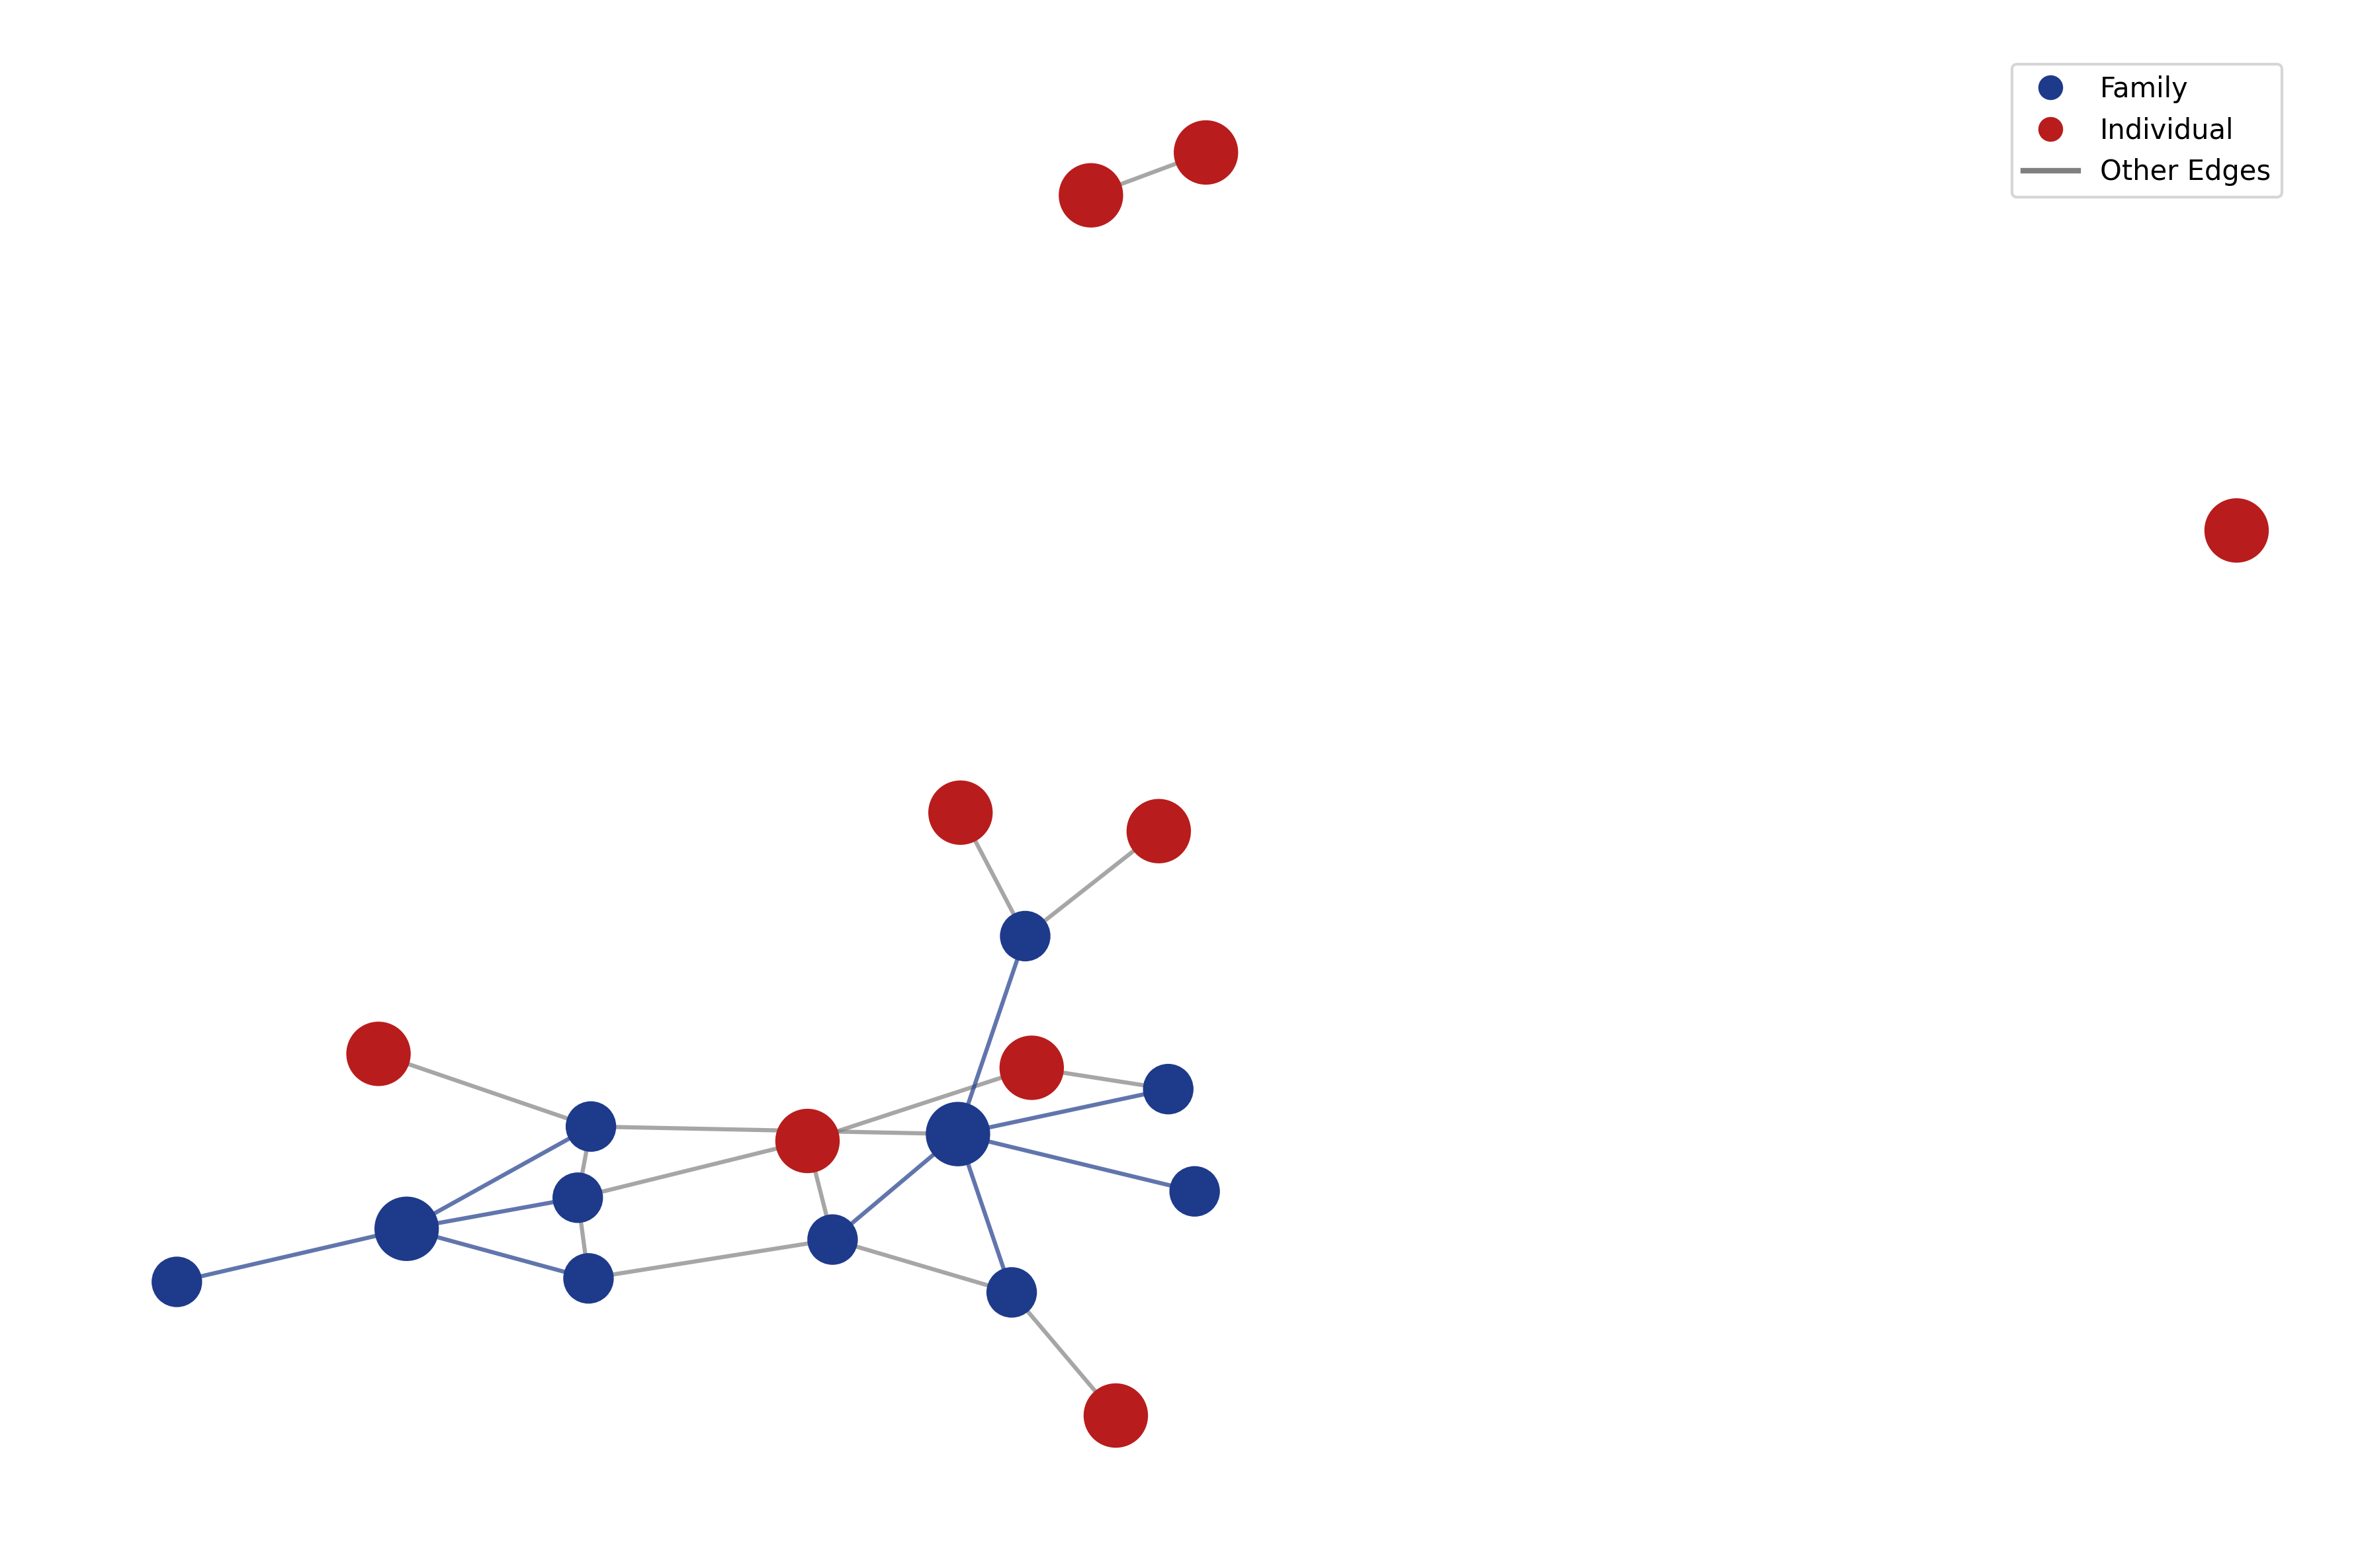
\includegraphics[width=0.48\linewidth]{assets/figures/graph_random_20.png}
  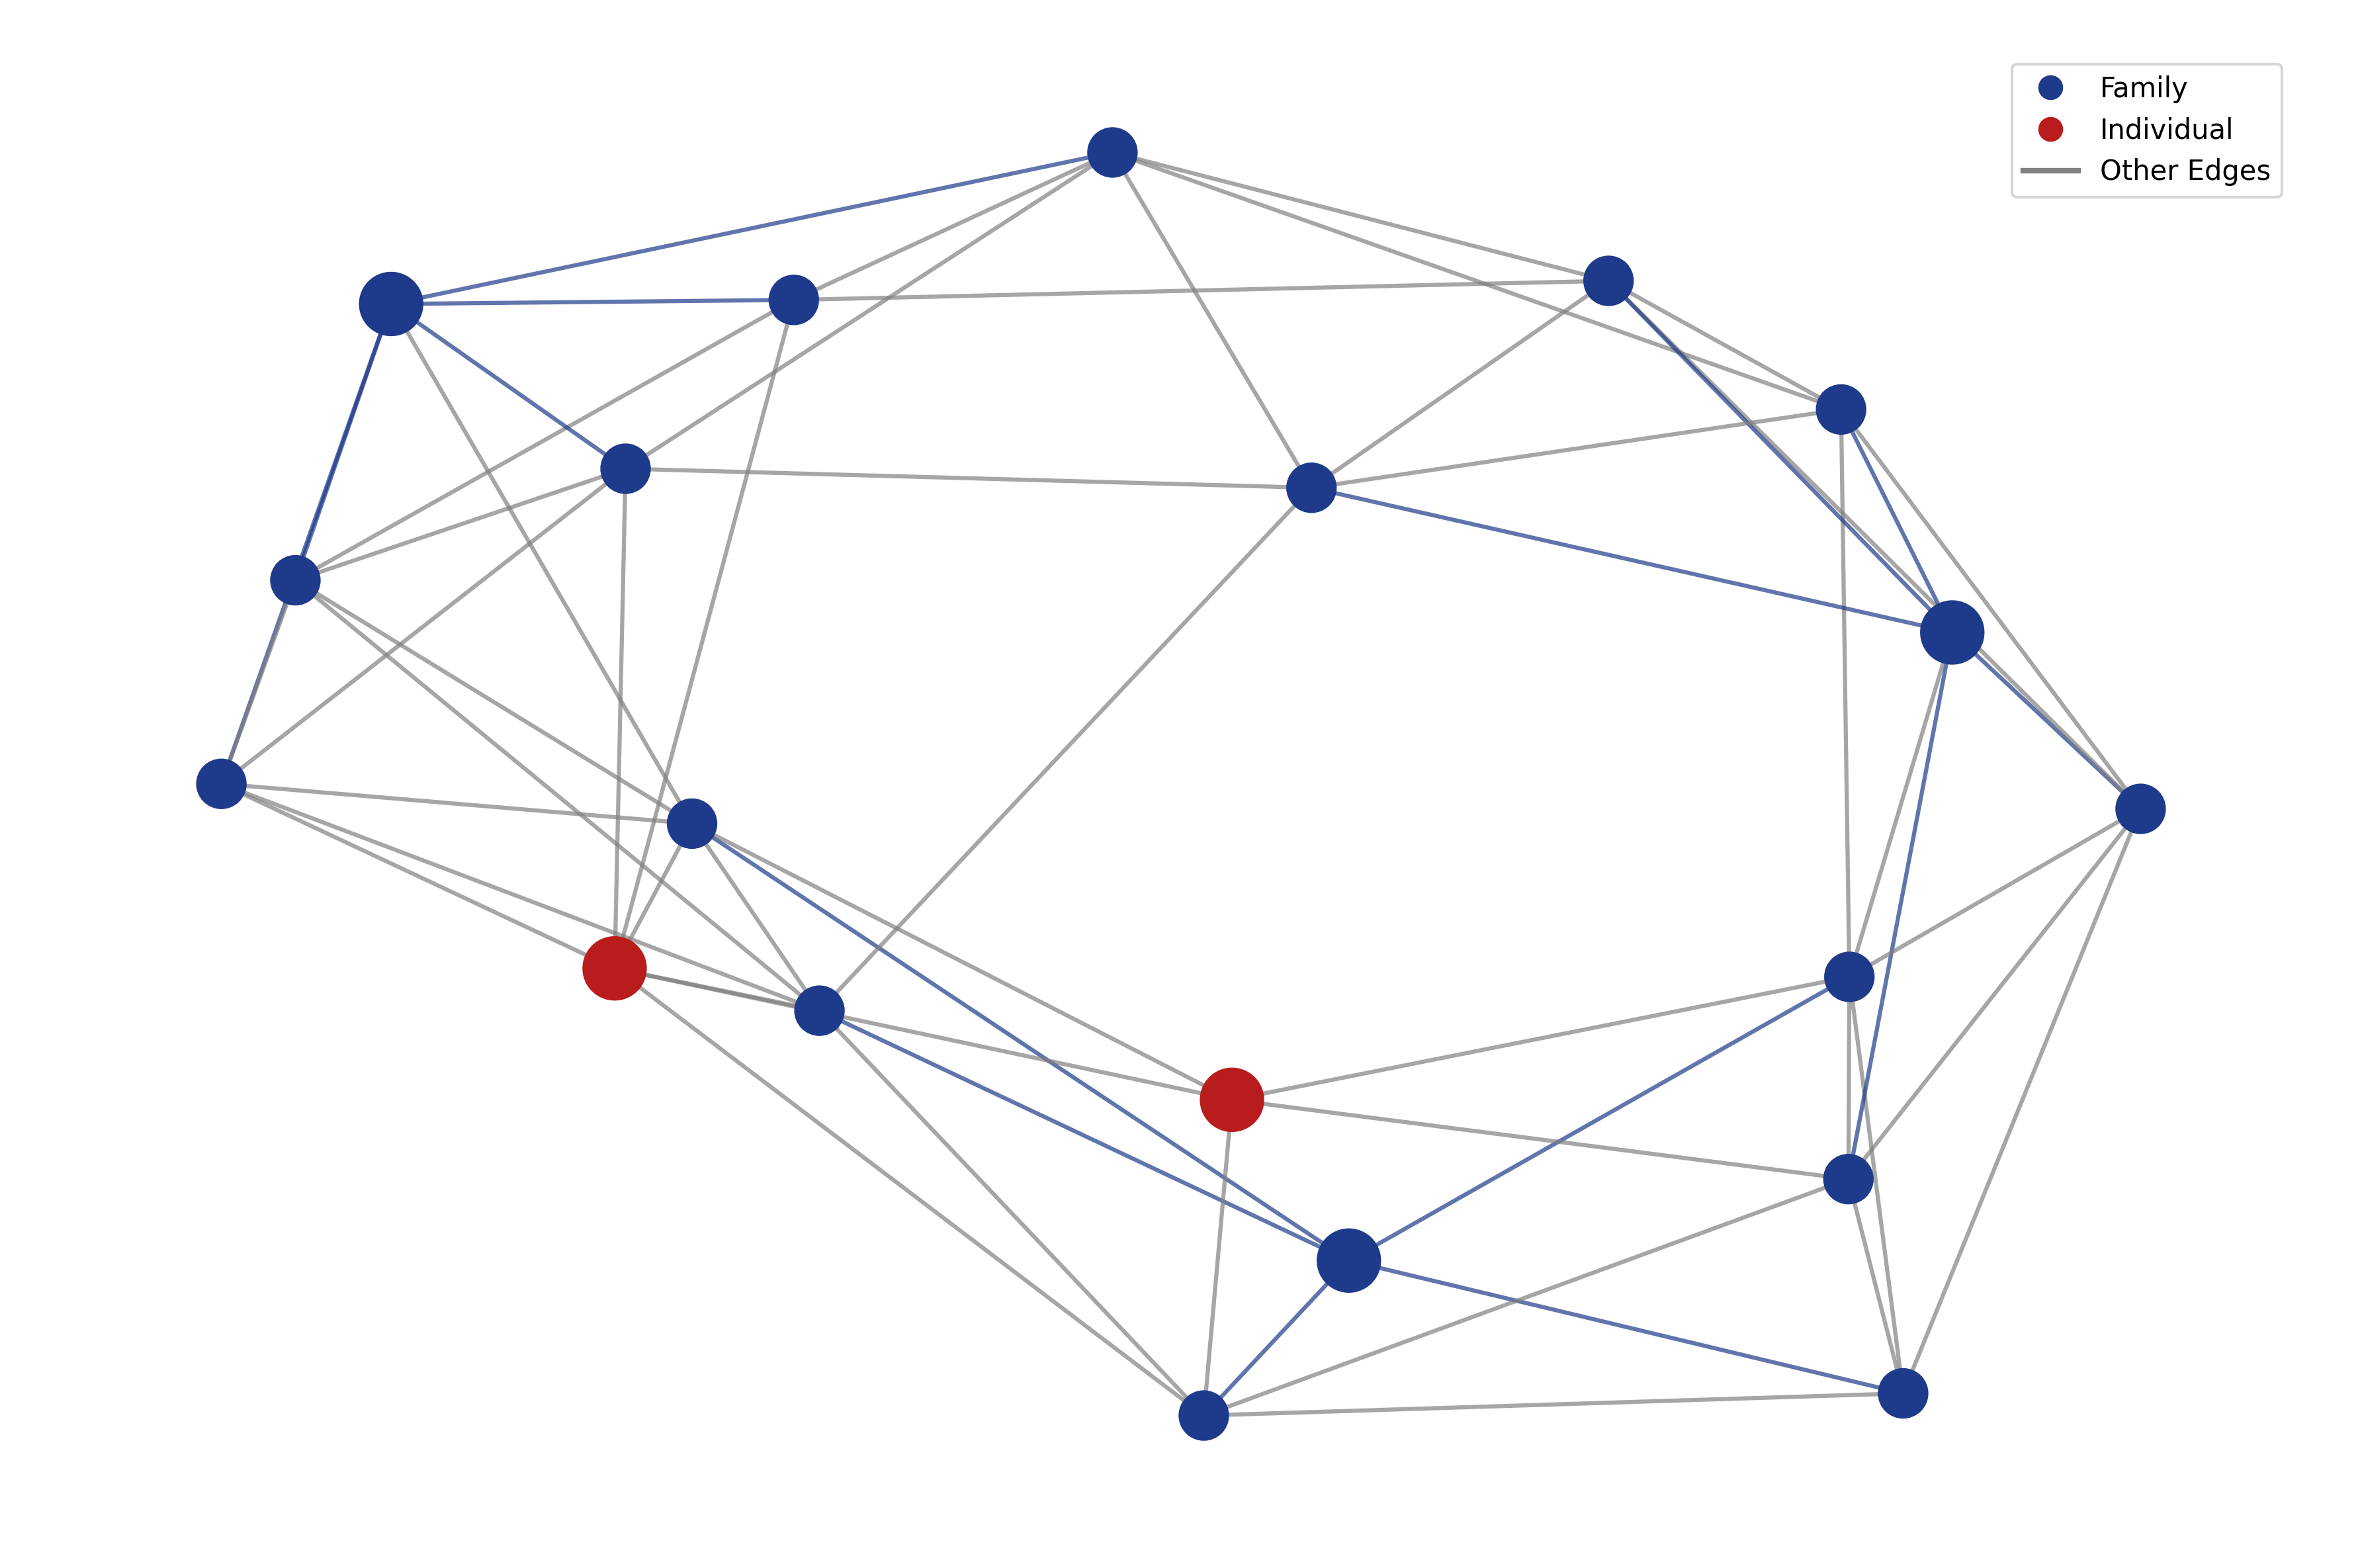
\includegraphics[width=0.48\linewidth]{assets/figures/graph_small_world_20.png}
  \caption{Przykładowe grafy syntetyczne: losowy (lewy) i małoświatowy (prawy).}
  \label{fig:graphs_synthetic}
\end{figure}

\begin{figure}[H]
  \centering
  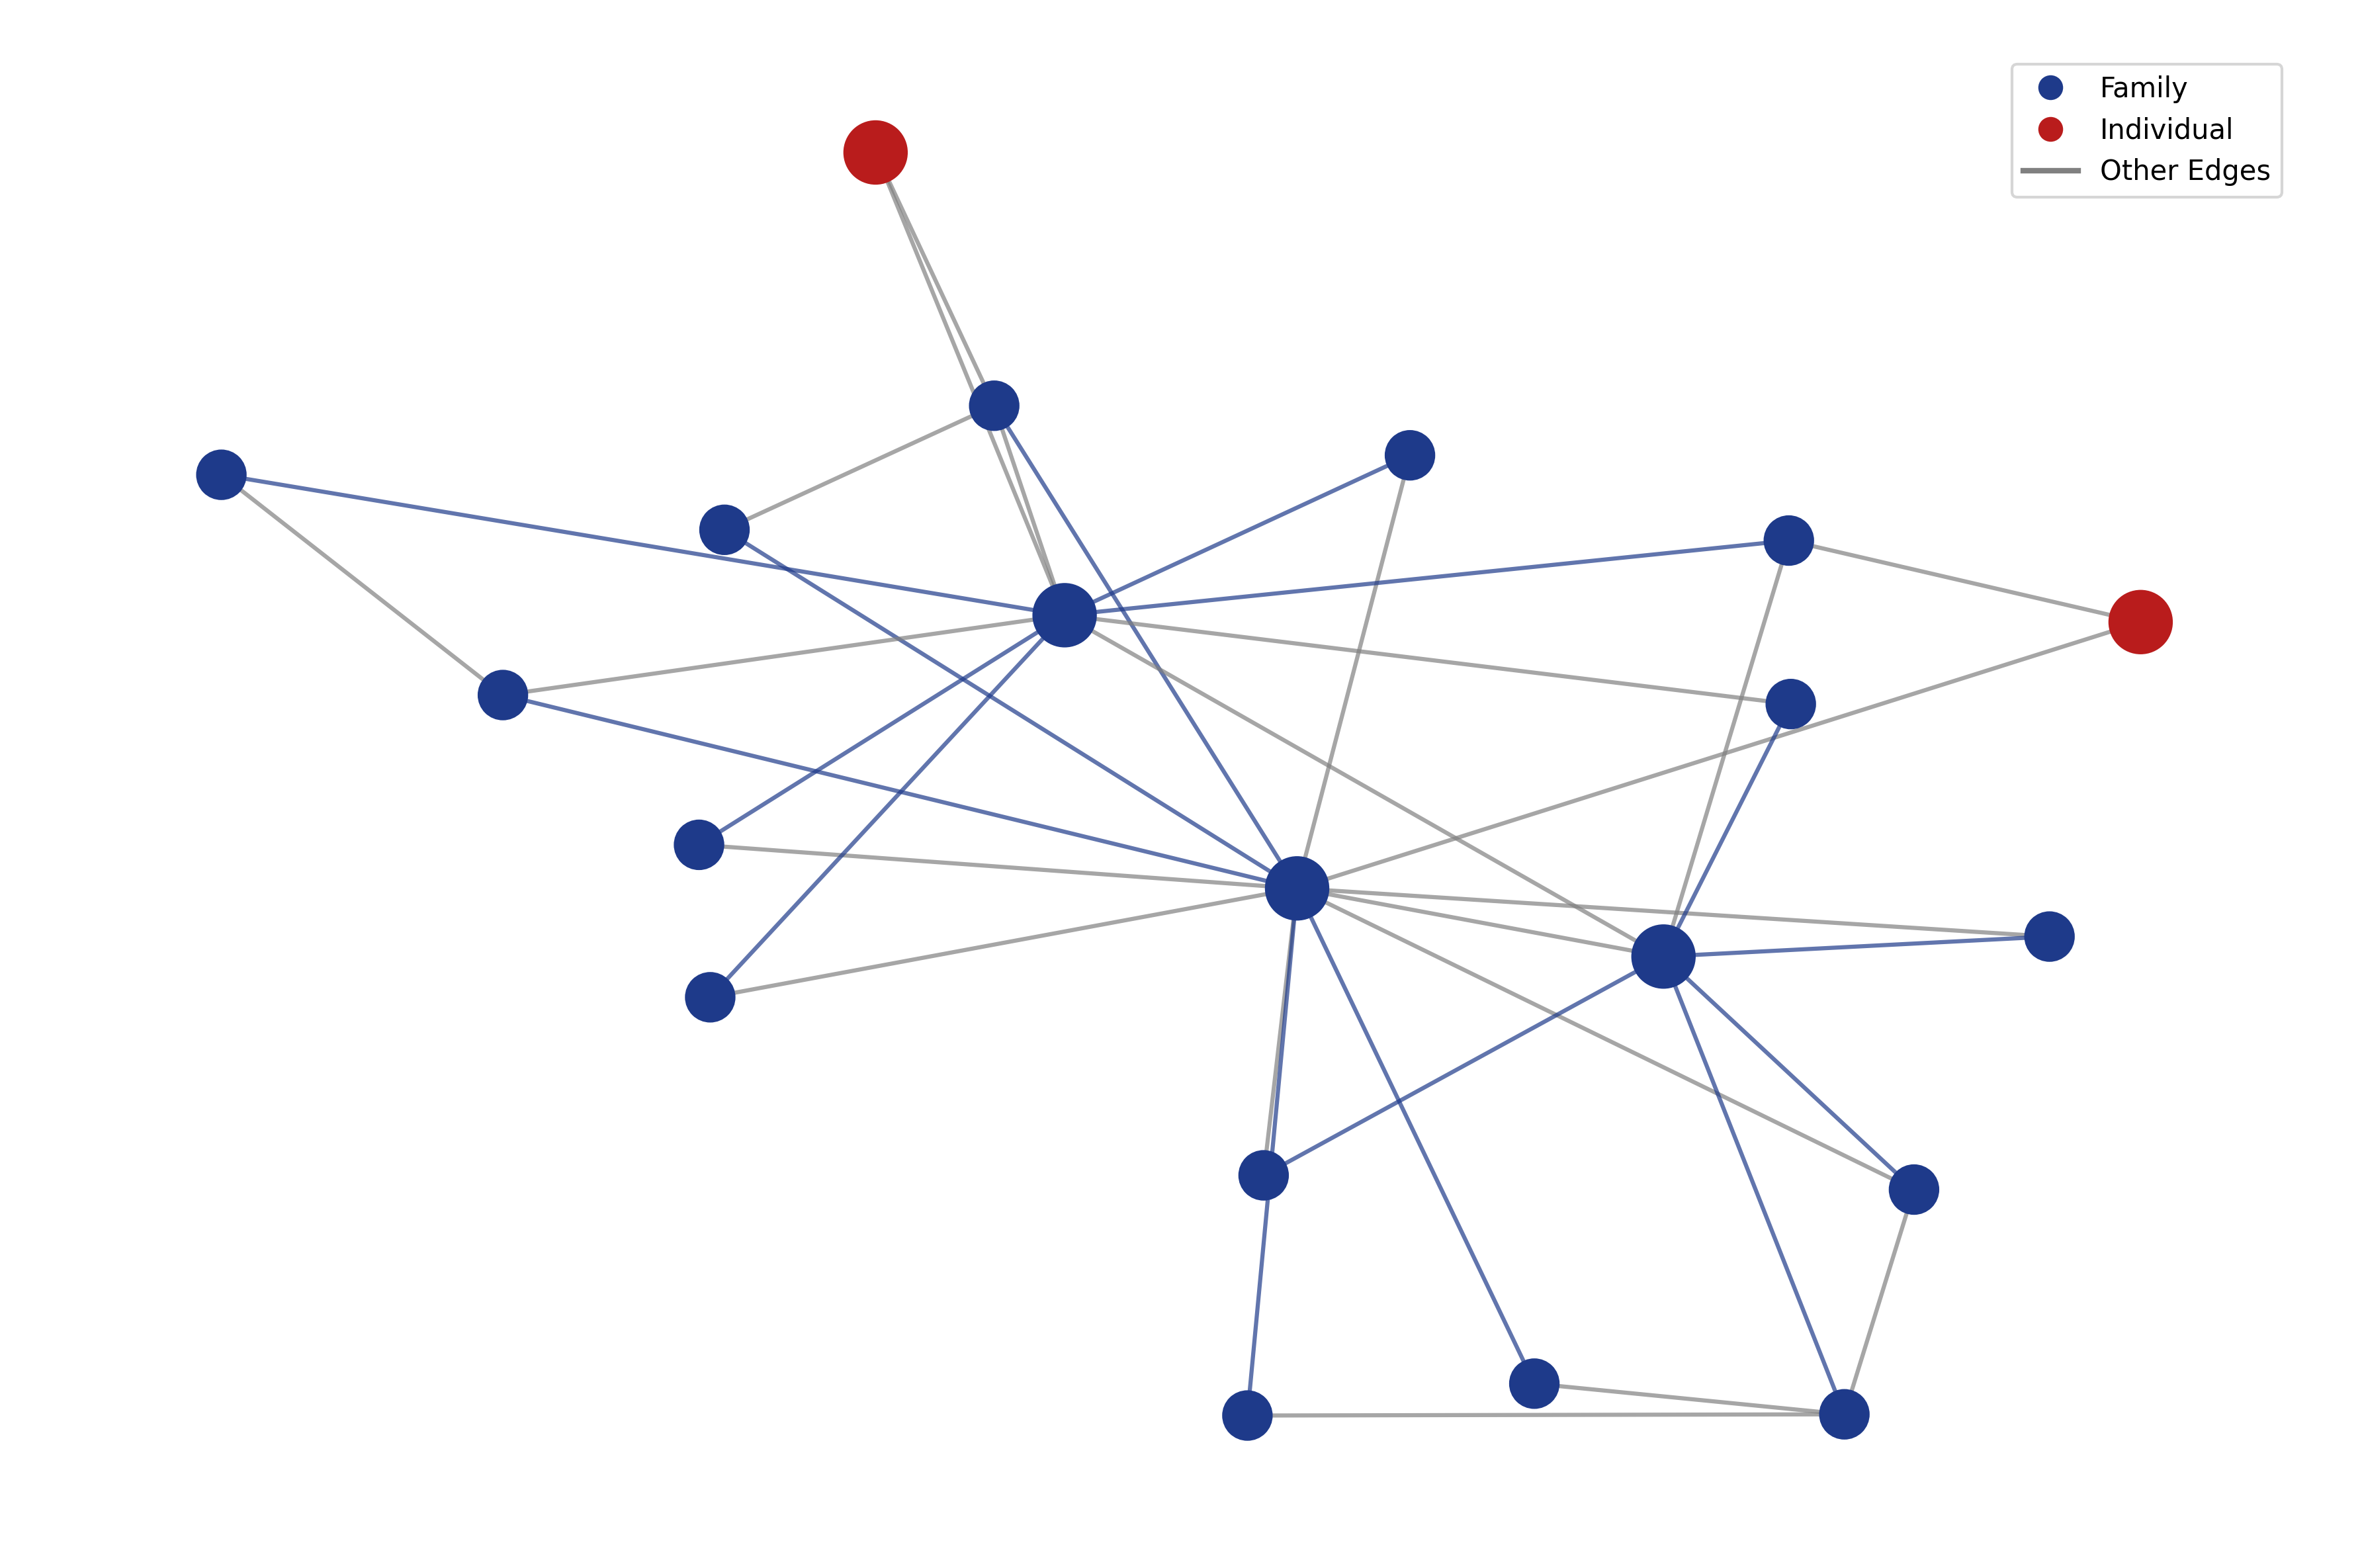
\includegraphics[width=0.48\linewidth]{assets/figures/graph_scale_free_20.png}
  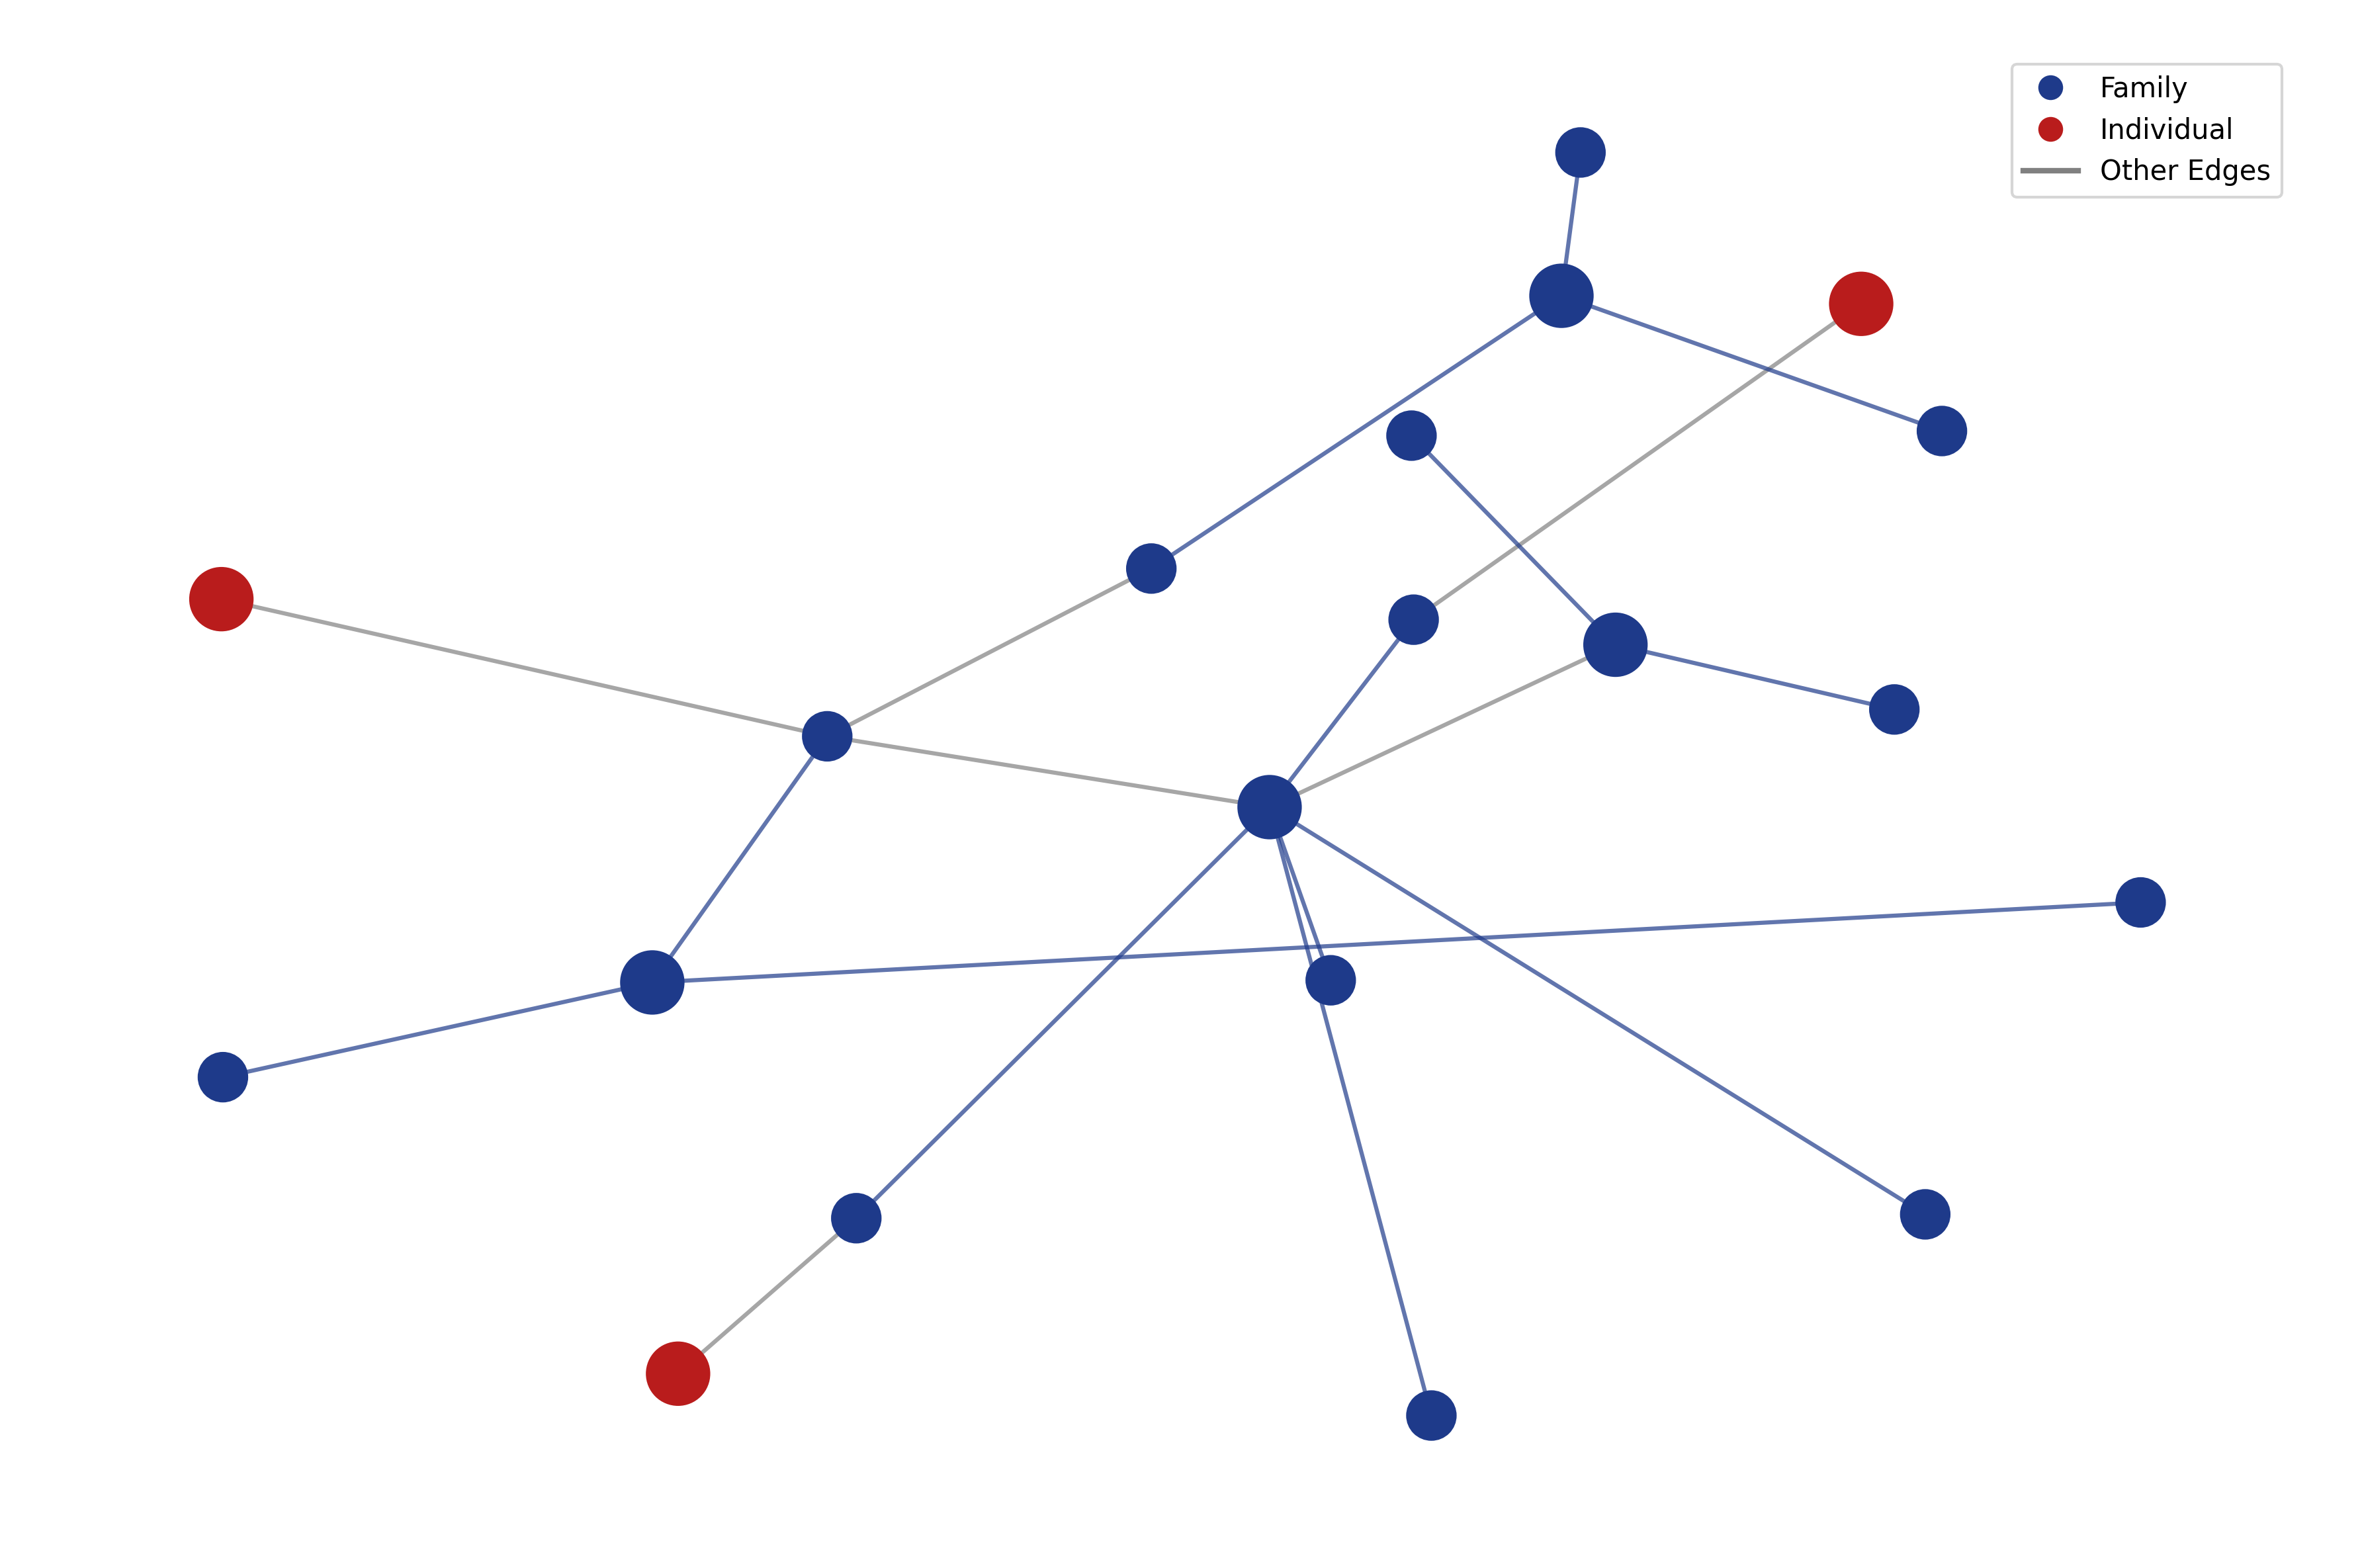
\includegraphics[width=0.48\linewidth]{assets/figures/graph_tree_20.png}
  \caption{Graf bezskalowy (lewy) i drzewo (prawy).}
  \label{fig:graphs_scale_tree}
\end{figure}

\begin{figure}[H]
  \centering
  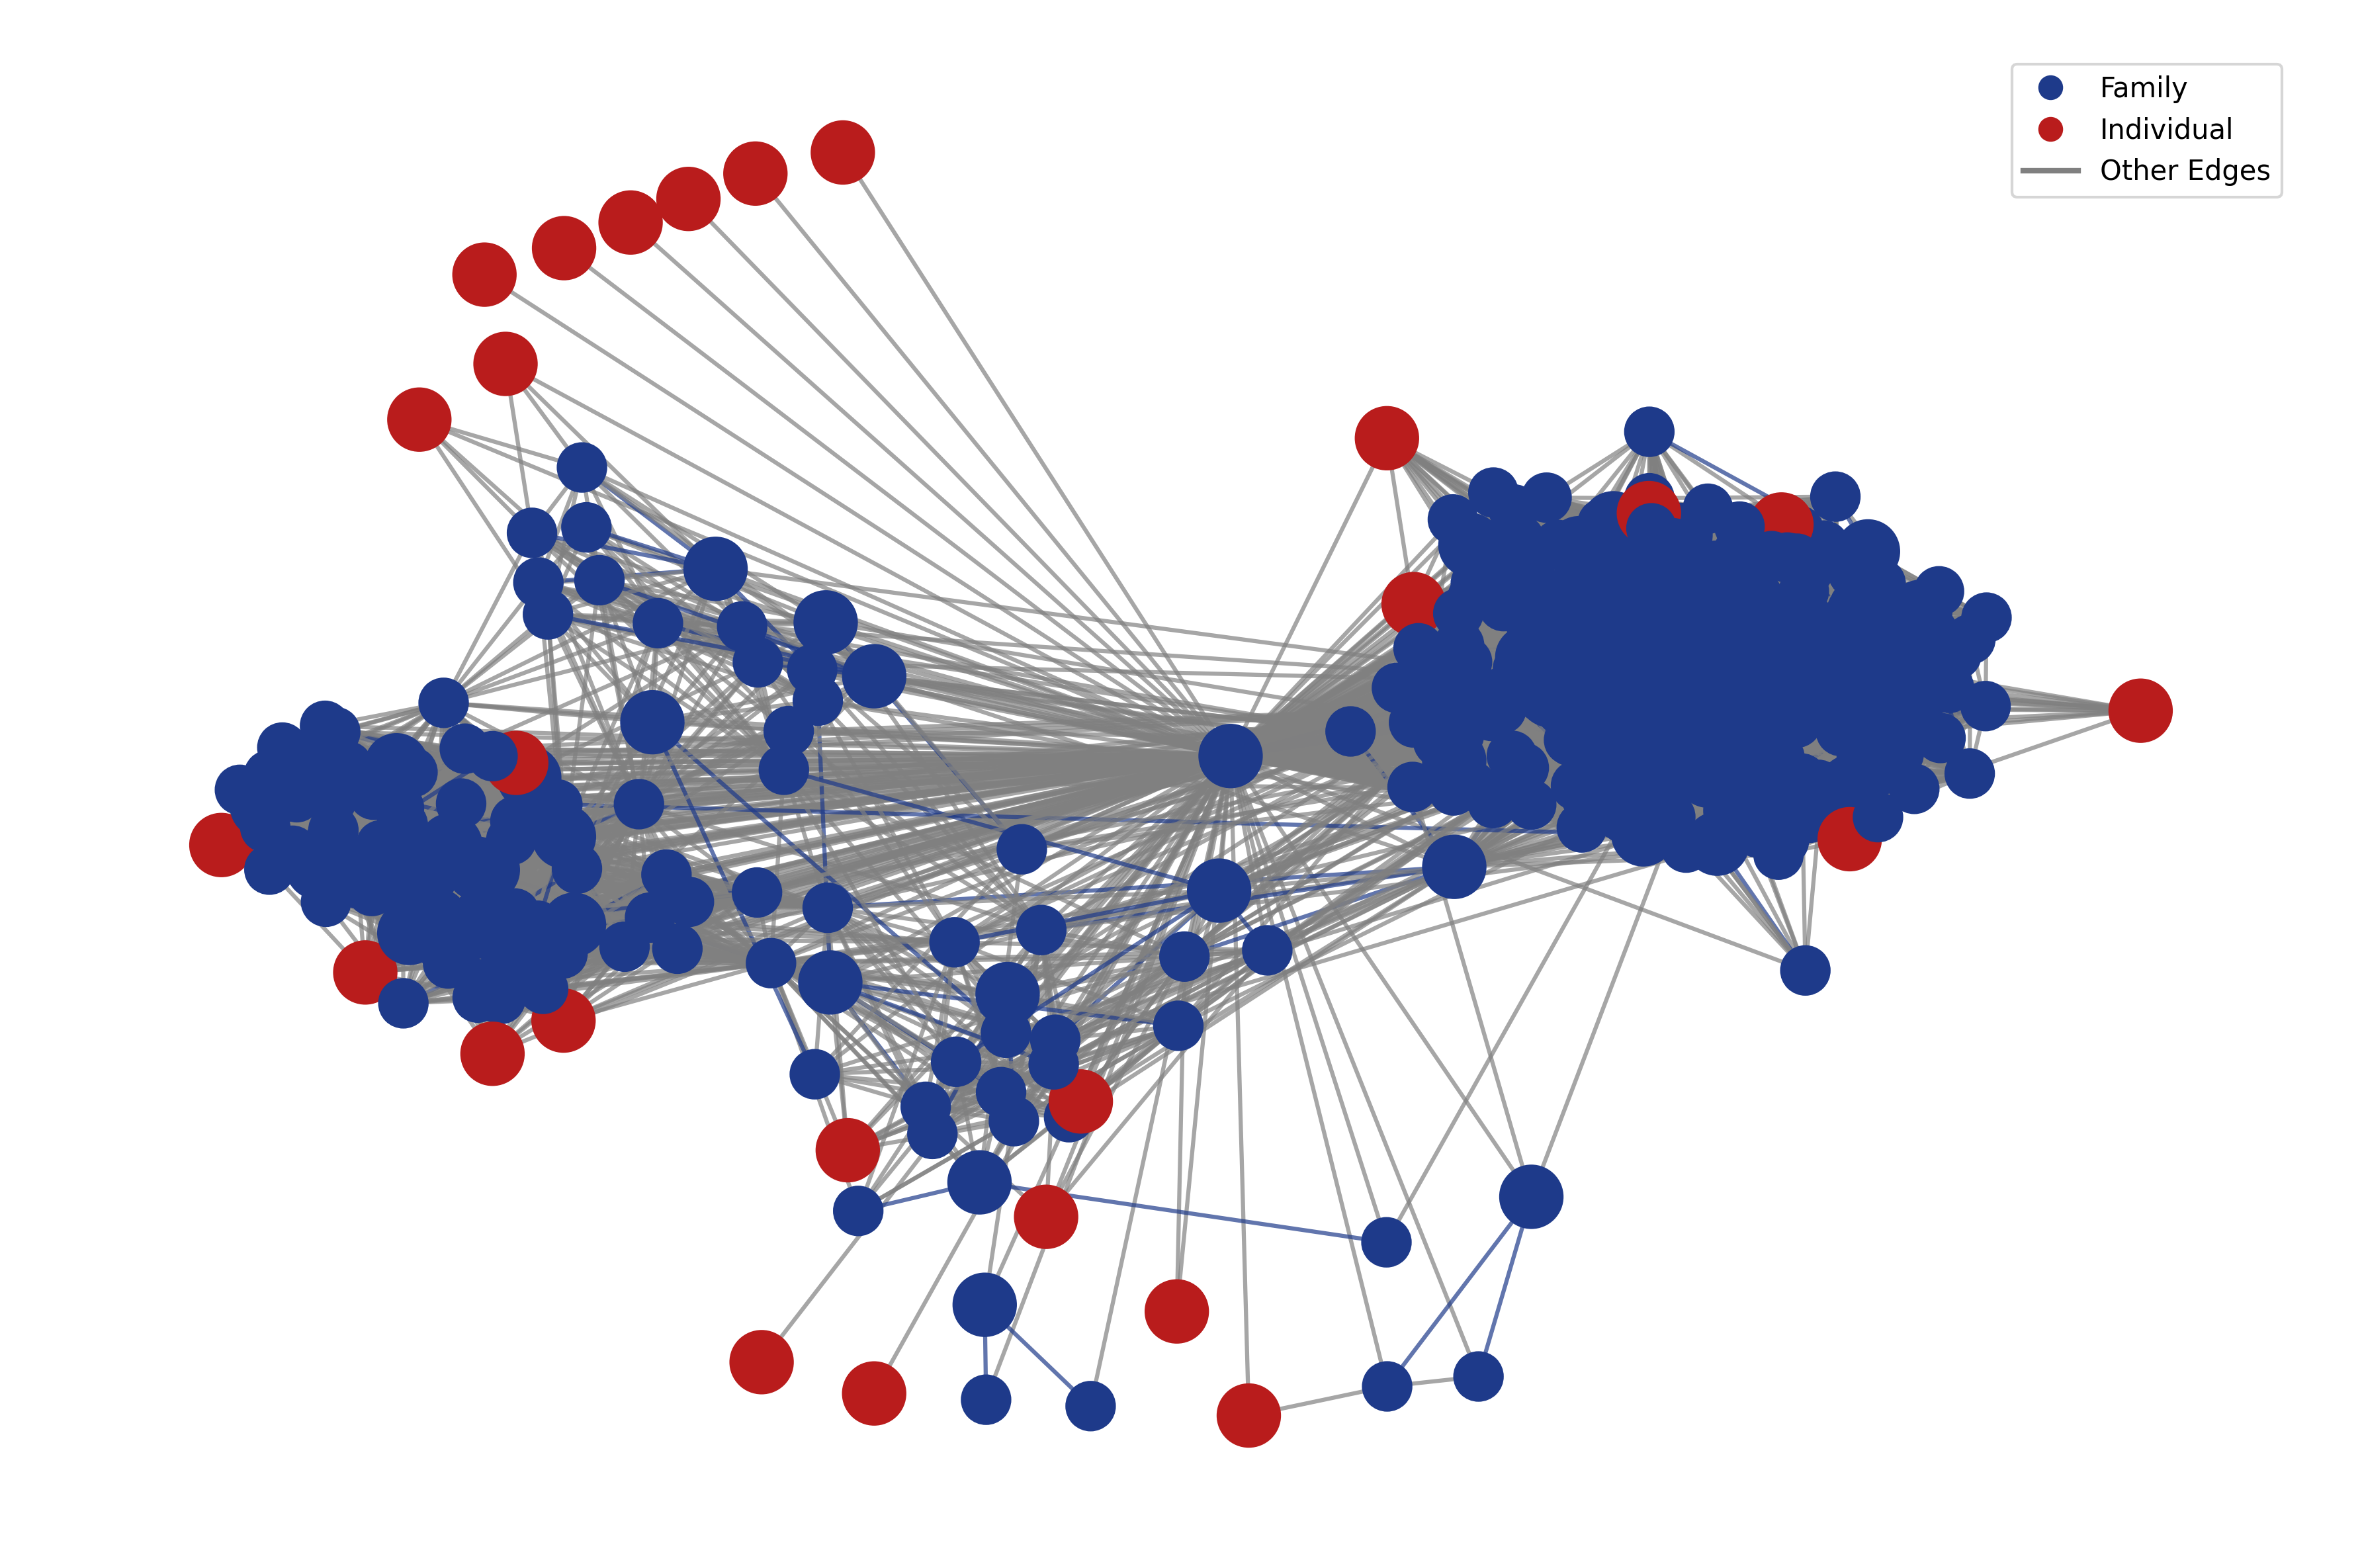
\includegraphics[width=0.6\linewidth]{assets/figures/graph_facebook_ego_107.png}
  \caption{Przykład rzeczywistej sieci Facebook ego (użytkownik 107).}
  \label{fig:graph_facebook}
\end{figure}

Widać wyraźne różnice w strukturze:
\begin{itemize}
  \item Grafy losowe mają równomiernie rozłożone połączenia
  \item Grafy małoświatowe tworzą lokalne skupienia z kilkoma długimi połączeniami
  \item Grafy bezskalowe mają wyraźne huby (wierzchołki o bardzo wysokim stopniu)
  \item Sieci Facebook są naturalnymi przykładami małoświatowych struktur społecznościowych
\end{itemize}

\section{Wyniki eksperymentów}

\subsection{Wydajność algorytmów dla konfiguracji duolingo\_super}

Na wykresach poniżej przedstawiono zachowanie różnych algorytmów dla konfiguracji licencji duolingo\_super na grafach syntetycznych.

\begin{figure}[H]
  \centering
  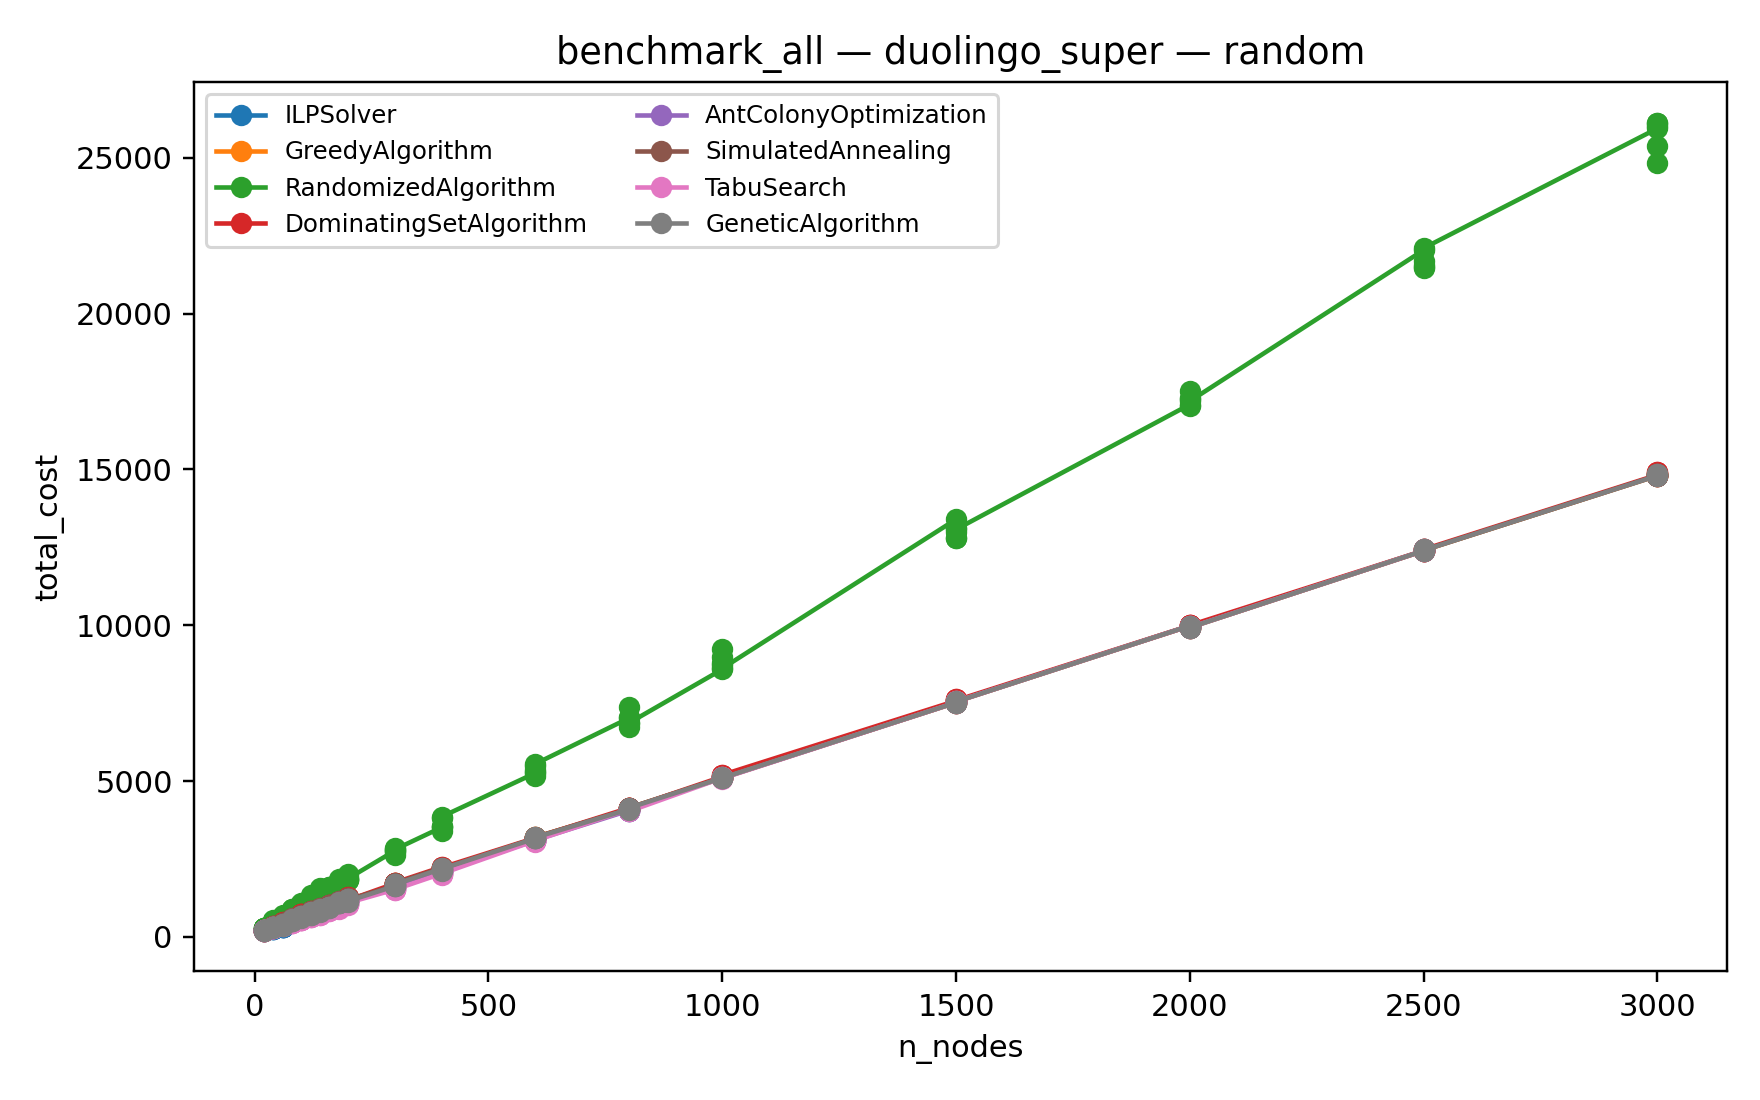
\includegraphics[width=0.48\linewidth]{assets/figures/ba_random_duo_cost_vs_n.png}
  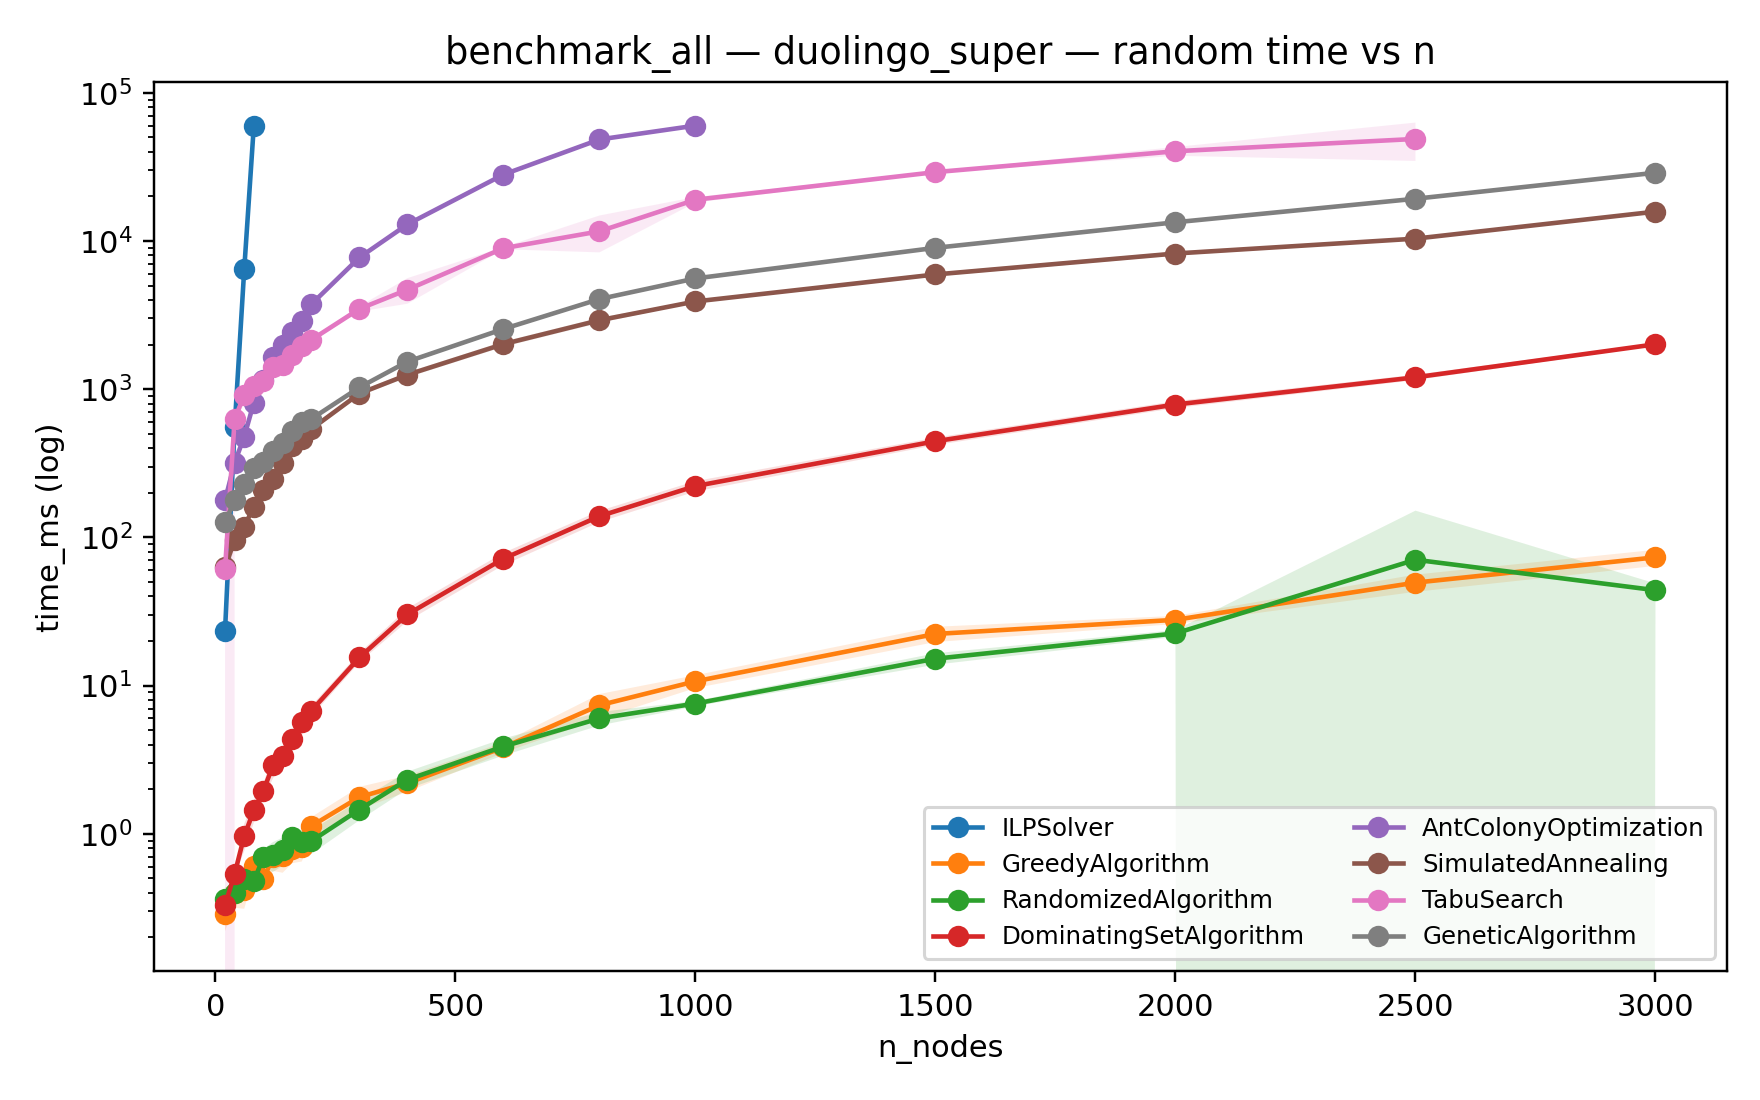
\includegraphics[width=0.48\linewidth]{assets/figures/ba_random_duo_time_vs_n.png}
  \caption{Grafy losowe (konf. duolingo\_super) -- koszt na wierzchołek i czas wykonania vs liczba wierzchołków.}
  \label{fig:random_performance}
\end{figure}

\begin{figure}[H]
  \centering
  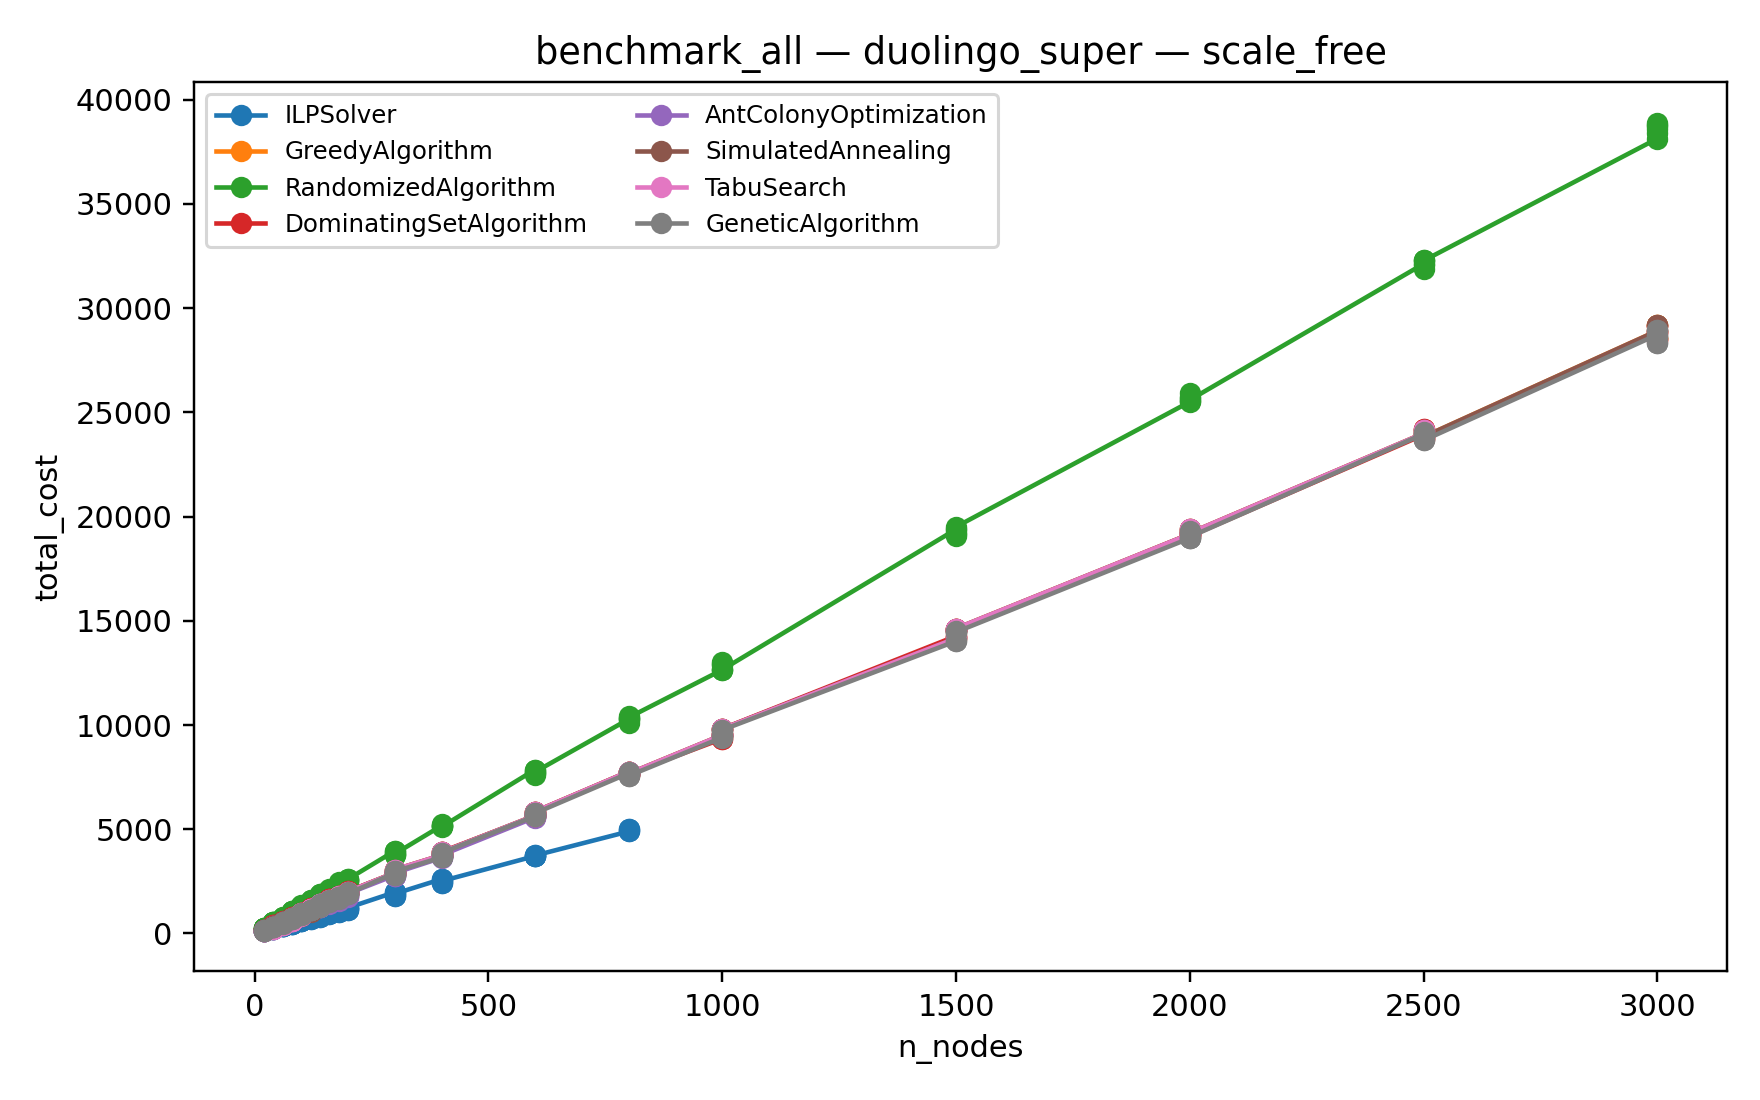
\includegraphics[width=0.48\linewidth]{assets/figures/ba_scale_free_duo_cost_vs_n.png}
  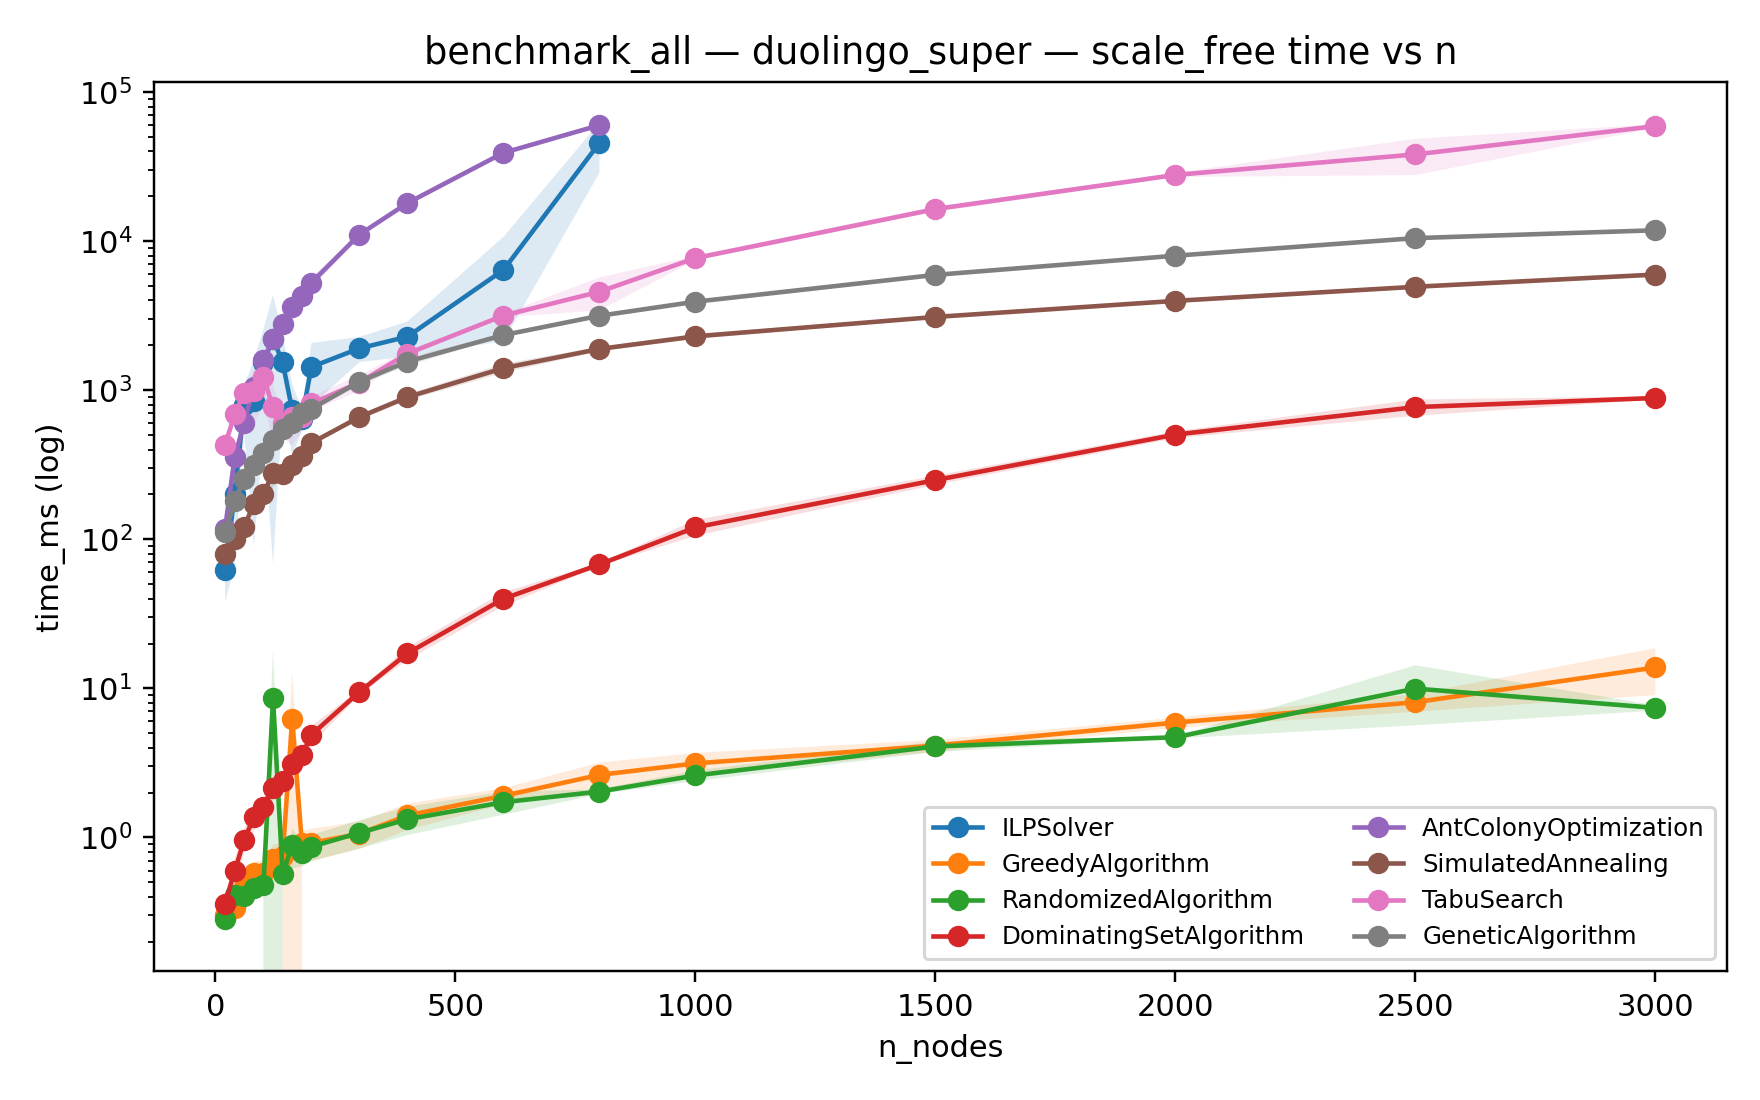
\includegraphics[width=0.48\linewidth]{assets/figures/ba_scale_free_duo_time_vs_n.png}
  \caption{Grafy bezskalowe (konf. duolingo\_super) -- koszt na wierzchołek i czas wykonania vs liczba wierzchołków.}
  \label{fig:scale_free_performance}
\end{figure}

\begin{figure}[H]
  \centering
  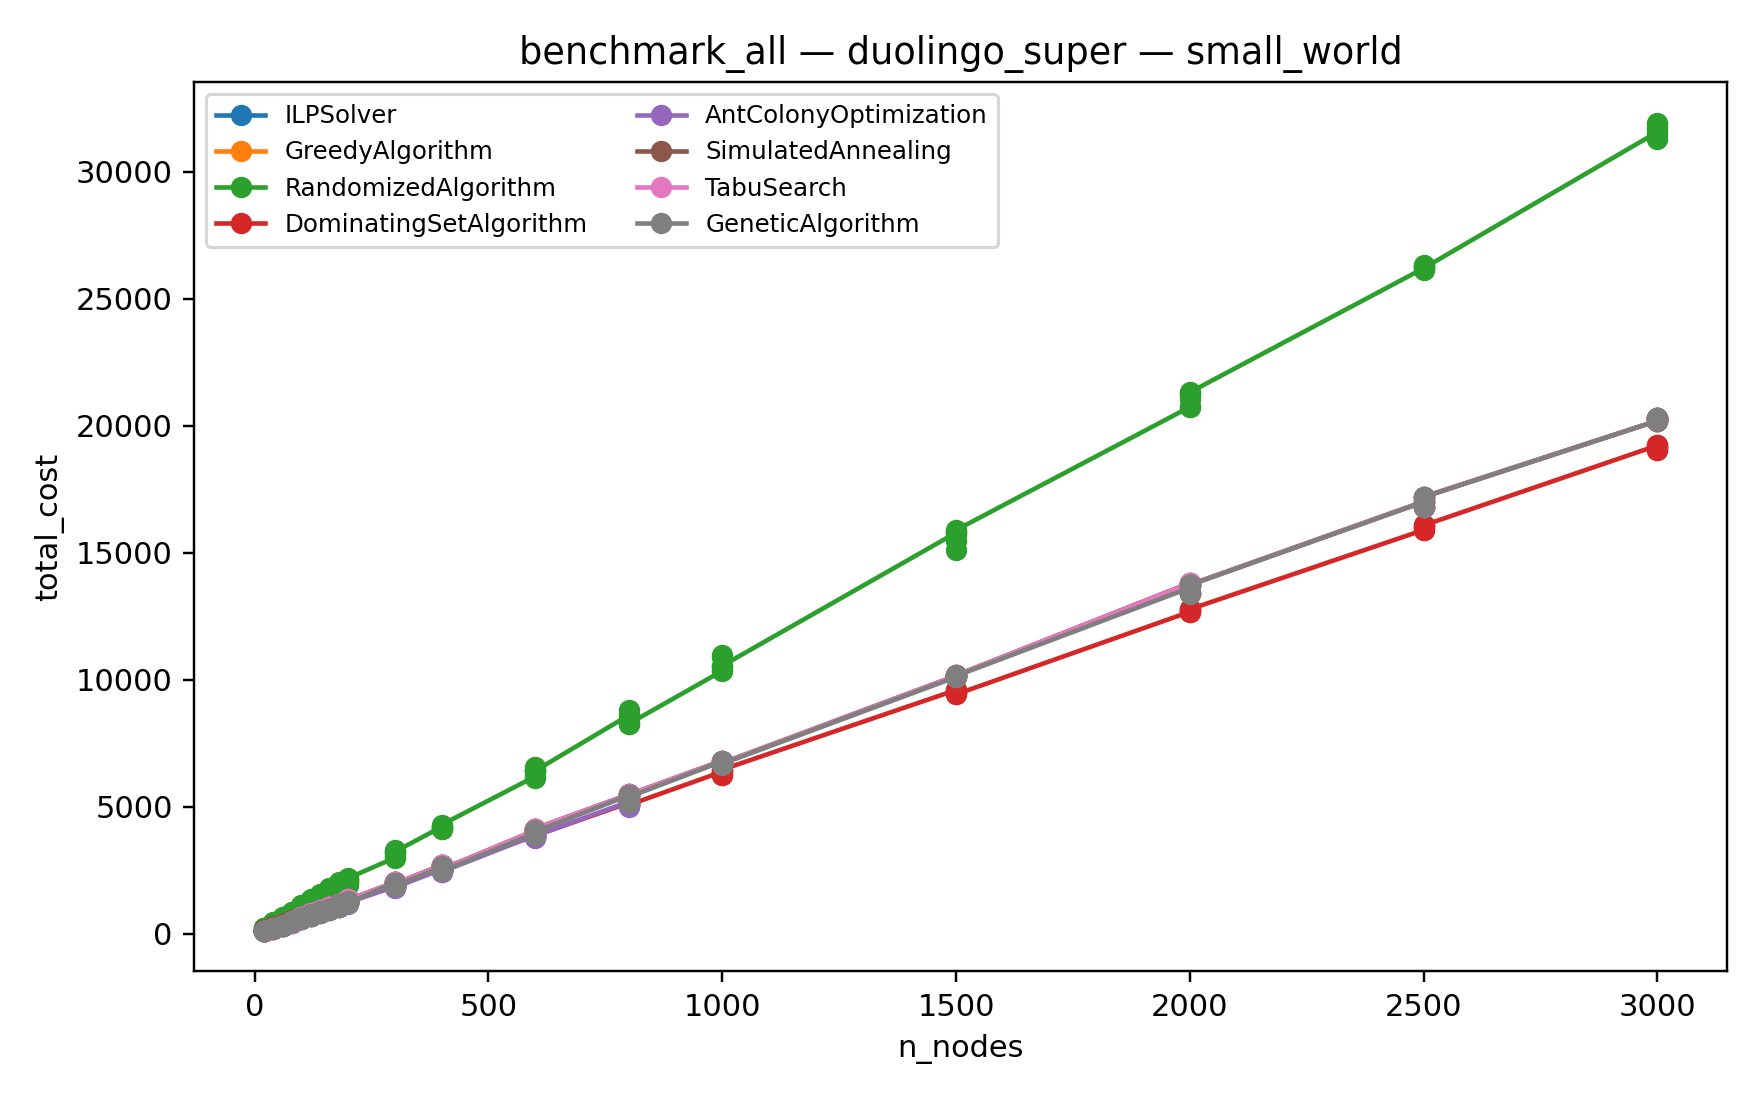
\includegraphics[width=0.48\linewidth]{assets/figures/ba_small_world_duo_cost_vs_n.png}
  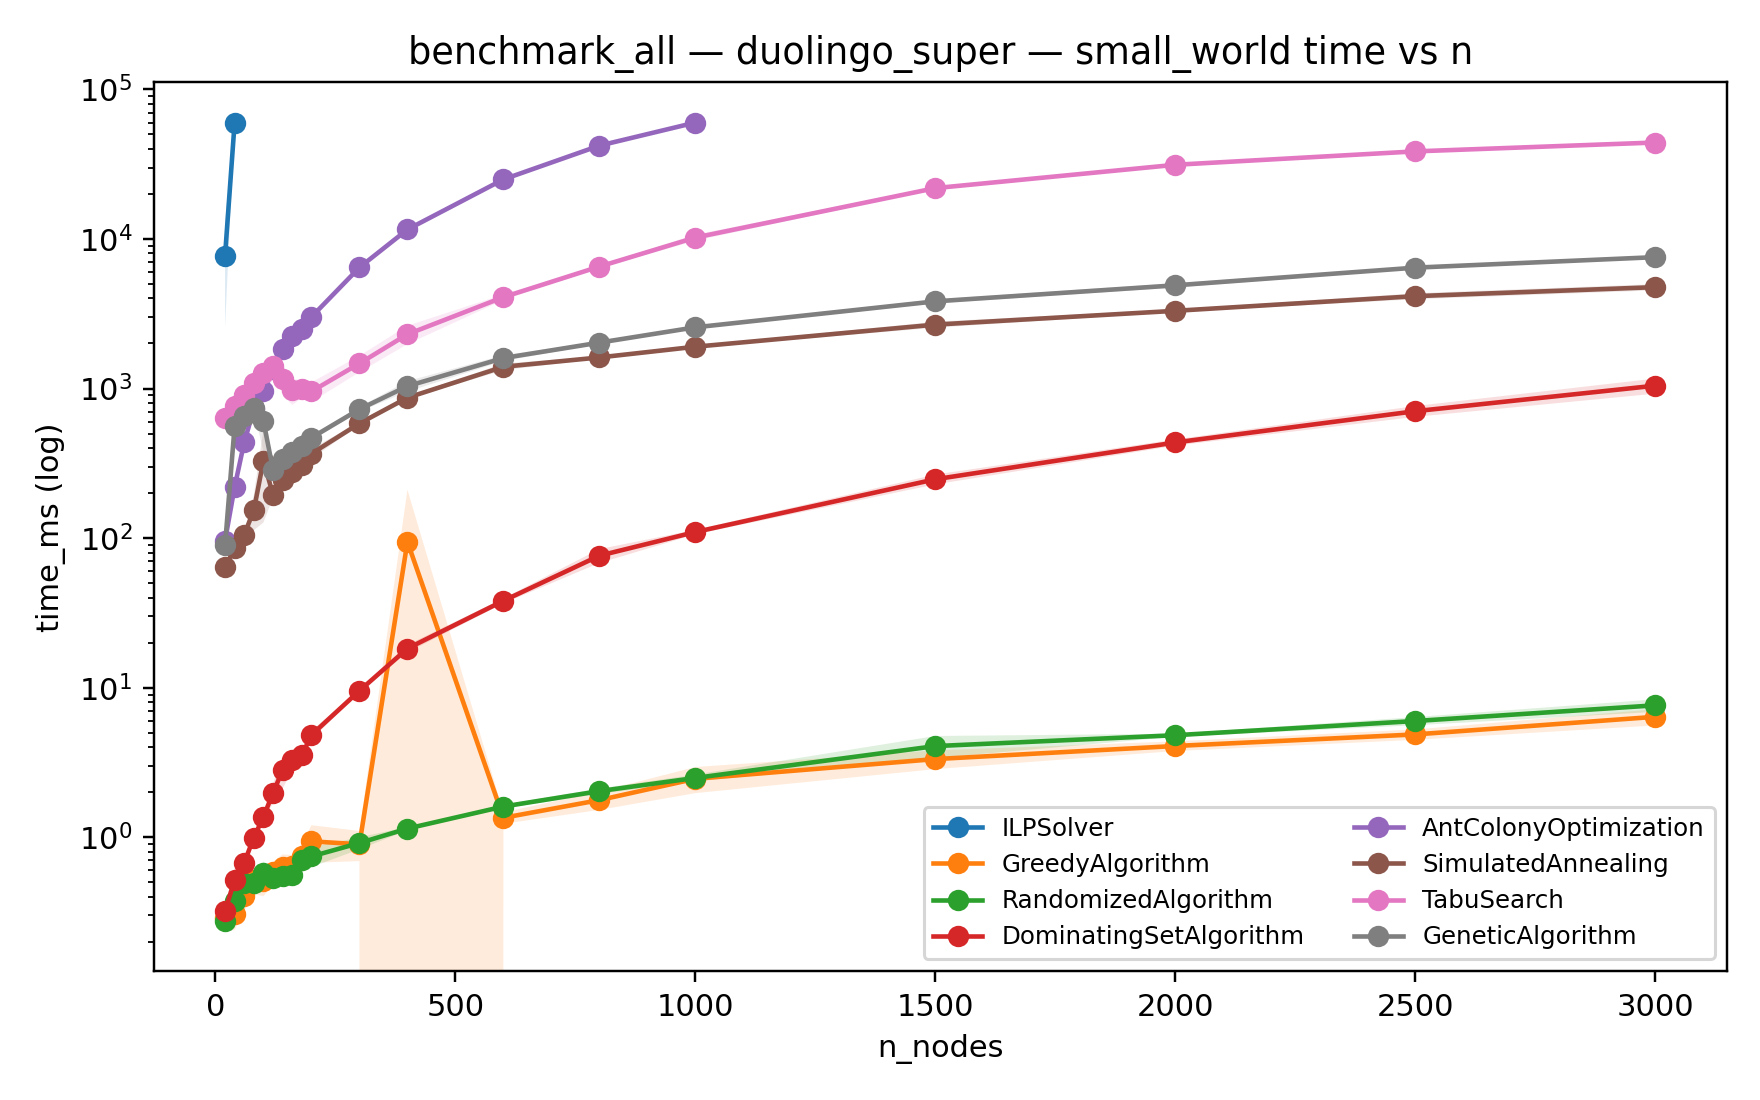
\includegraphics[width=0.48\linewidth]{assets/figures/ba_small_world_duo_time_vs_n.png}
  \caption{Grafy małoświatowe (konf. duolingo\_super) -- koszt na wierzchołek i czas wykonania vs liczba wierzchołków.}
  \label{fig:small_world_performance}
\end{figure}

Z wykresów wynika kilka ważnych obserwacji:

\paragraph{Jakość rozwiązań}
Metaheurystyki (algorytm genetyczny, symulowane wyżarzanie, tabu search, ant colony) dają najniższe koszty, ale są znacznie wolniejsze. Algorytm zachłanny (greedy) oferuje dobry kompromis -- jest szybki i daje wyniki tylko nieznacznie gorsze niż metaheurystyki.

\paragraph{Czas wykonania}
ILP bardzo szybko staje się niepraktyczny -- już dla grafów powyżej 100-200 wierzchołków przekracza limit czasu 60 sekund. Heurystyki konstrukcyjne (greedy, random, dominating set) są bardzo szybkie nawet dla dużych grafów.

\paragraph{Wpływ struktury grafu}
Grafy bezskalowe pozwalają na niższe koszty niż losowe czy małoświatowe -- to dlatego, że huby umożliwiają tworzenie większych, bardziej efektywnych grup licencyjnych.

\subsection{Porównanie konfiguracji licencji}

Bezpośrednie porównanie kosztów między Duolingo Super (ceny rzeczywiste) a wariantem roman domination (koszty względne) nie jest miarodajne — różne skale cenowe w naturalny sposób przekładają się na różne średnie koszty. W tym rozdziale koncentrujemy się więc na trendach w obrębie danej konfiguracji (wpływ struktury grafu i \(n\)), a porównania wariantów modelu przedstawiamy w rozdz.\,\ref{chap:extensions} (np. krzywe roman\_p\_x, analiza Spotify).

\subsection{Analiza gęstości i struktury grafów}

\begin{figure}[H]
  \centering
  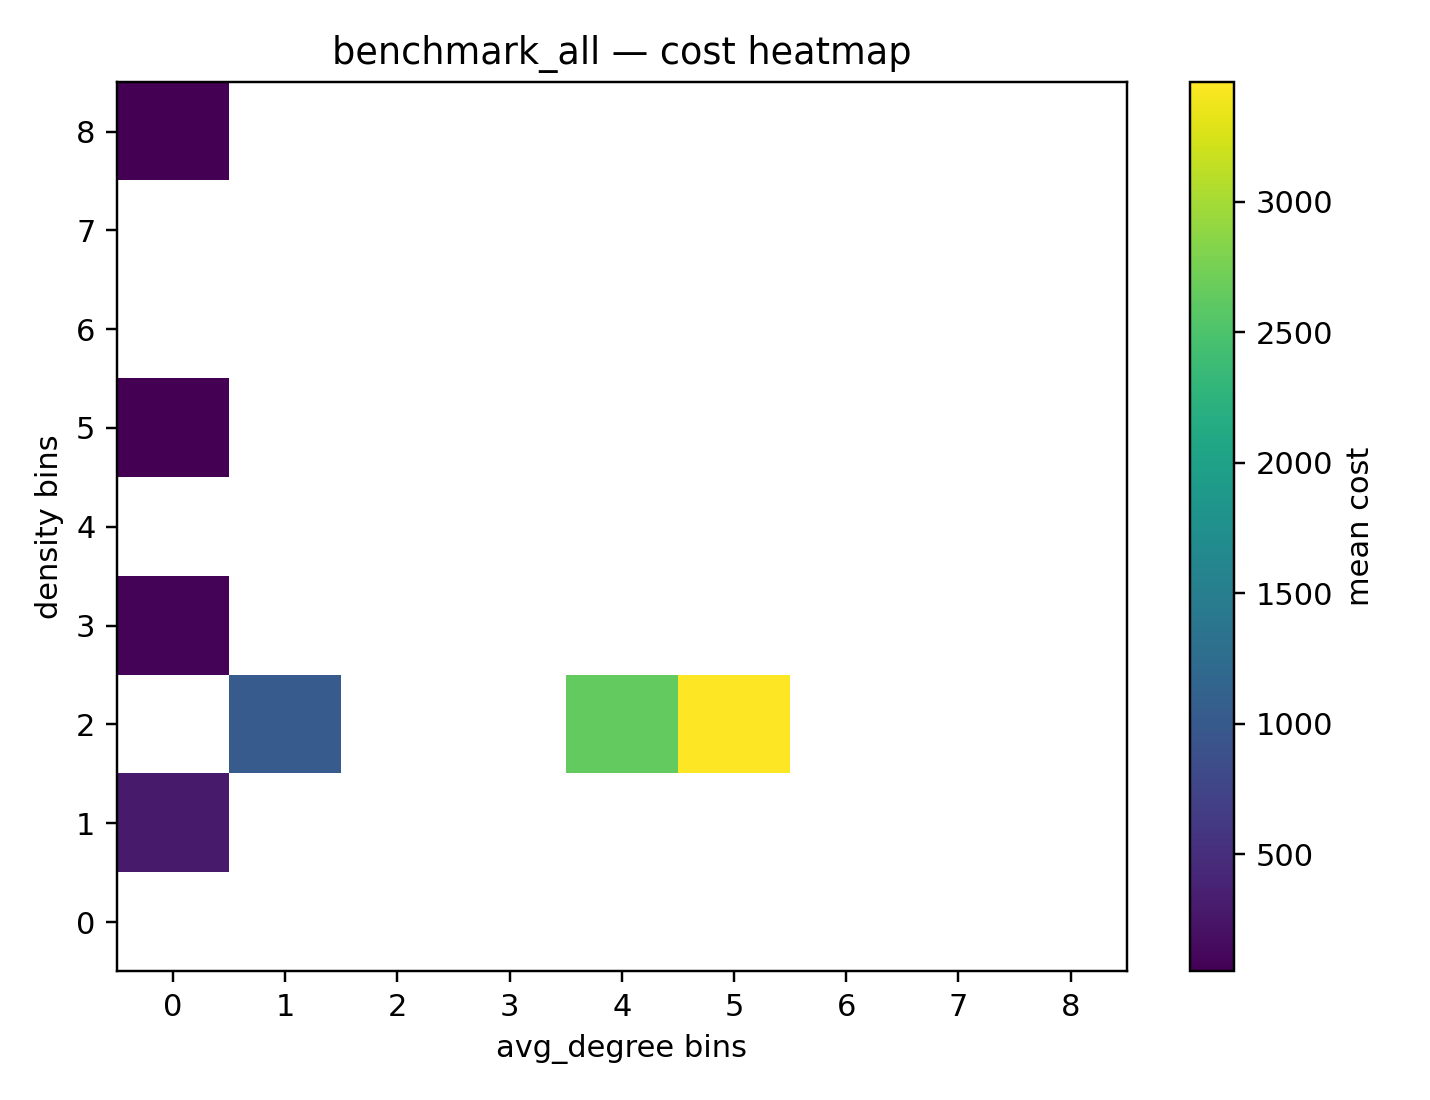
\includegraphics[width=0.7\linewidth]{assets/figures/ba_heatmap_cost.png}
  \caption{Heatmapa średniego kosztu na wierzchołek w zależności od gęstości i średniego stopnia grafu.}
  \label{fig:density_heatmap}
\end{figure}

% Zrezygnowano z dodatkowych wykresów gęstości (stare nazwy plików);
% wnioski omówiono na podstawie heatmapy.

Gęstość grafu ma kluczowy wpływ na koszty -- im więcej połączeń, tym łatwiej tworzyć duże grupy licencyjne, co obniża koszt na wierzchołek. Jednocześnie gęstsze grafy wymagają więcej czasu na obliczenia.

\subsection{Wykresy Pareto -- kompromis koszt vs czas}

Wykresy Pareto pokazują fronty niezdominowanych rozwiązań, gdzie żadne rozwiązanie nie jest jednocześnie tańsze i szybsze od innego.

\begin{figure}[H]
  \centering
  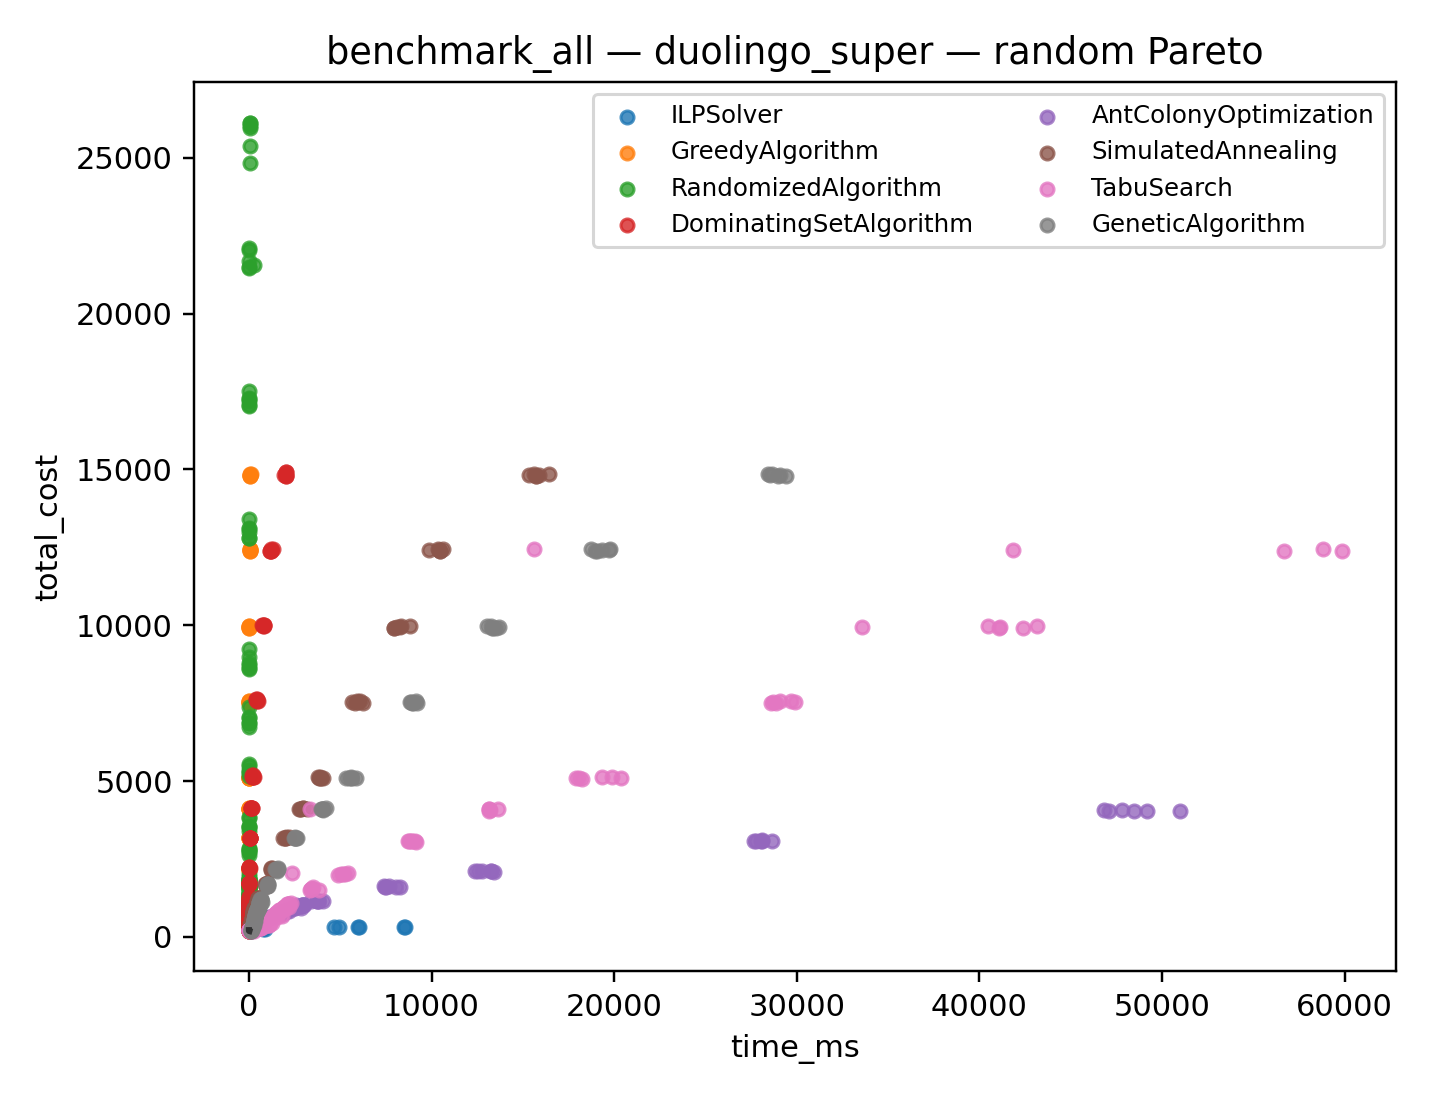
\includegraphics[width=0.48\linewidth]{assets/figures/ba_random_duo_pareto.png}
  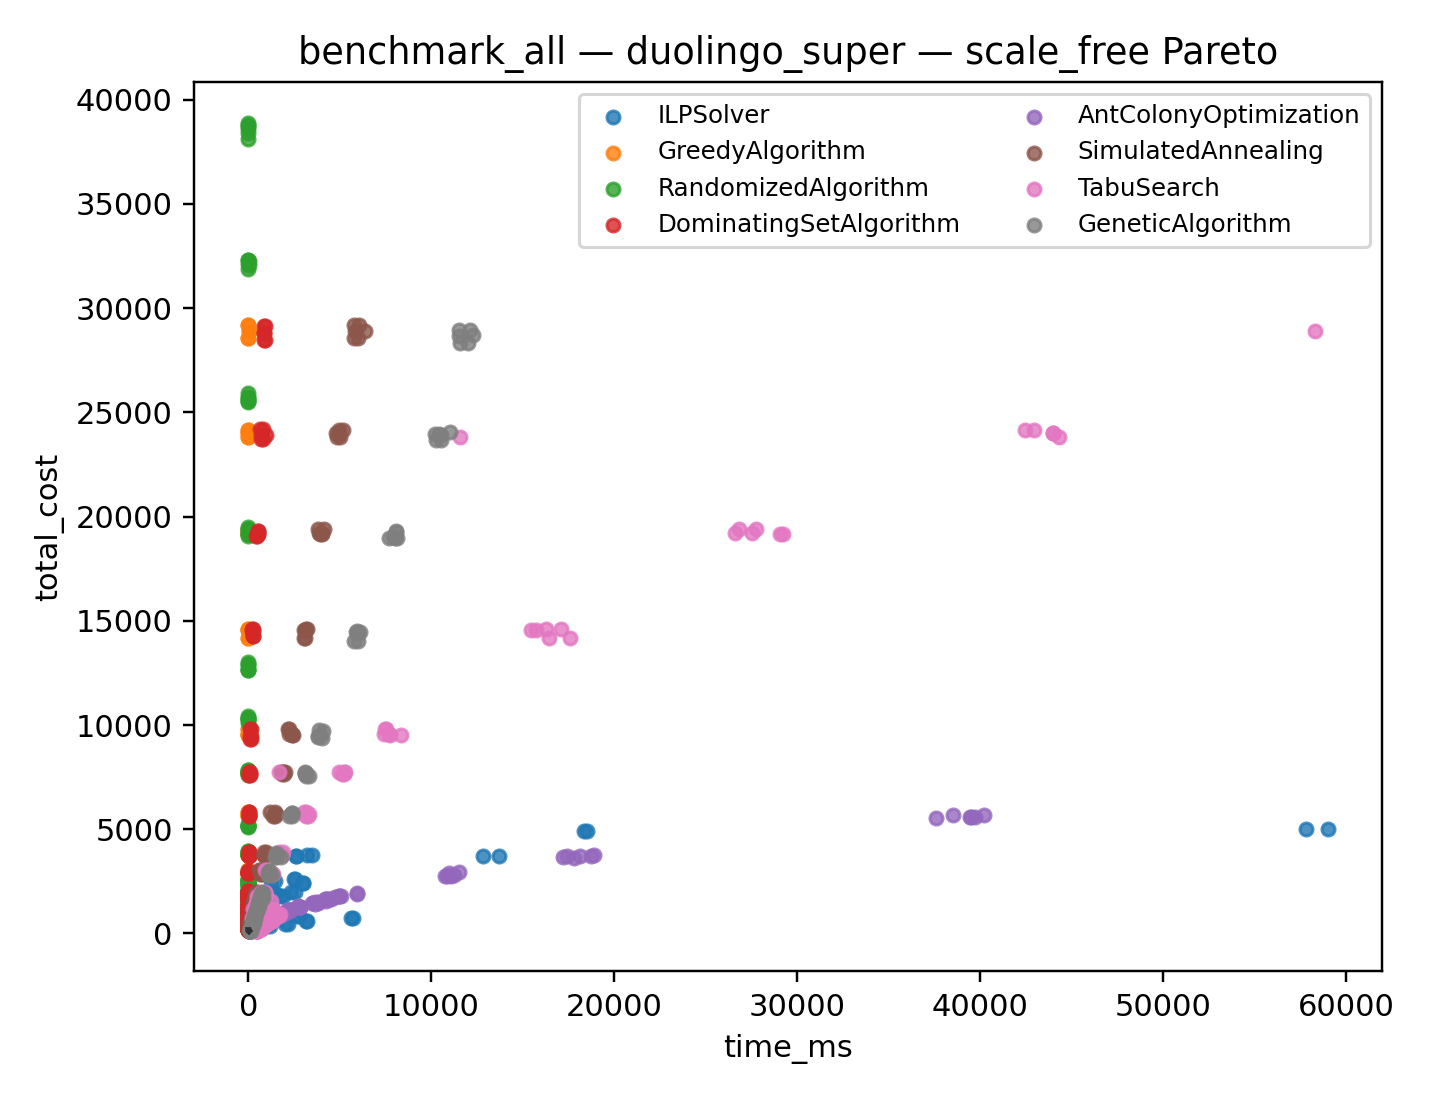
\includegraphics[width=0.48\linewidth]{assets/figures/ba_scale_free_duo_pareto.png}
  \caption{Fronty Pareto koszt vs czas dla grafów losowych (lewy) i bezskalowych (prawy), konf. duolingo\_super.}
  \label{fig:pareto_analysis}
\end{figure}

Na frontach Pareto widać:
\begin{itemize}
  \item Algorytm zachłanny oferuje najlepszy kompromis dla większości zastosowań
  \item ILP daje najniższy koszt, ale tylko dla małych grafów
  \item Metaheurystyki warto używać gdy czas nie jest krytyczny, a zależy nam na jak najniższym koszcie
\end{itemize}

\section{Wyniki dla grafów rzeczywistych}

\begin{figure}[h]
  \centering
  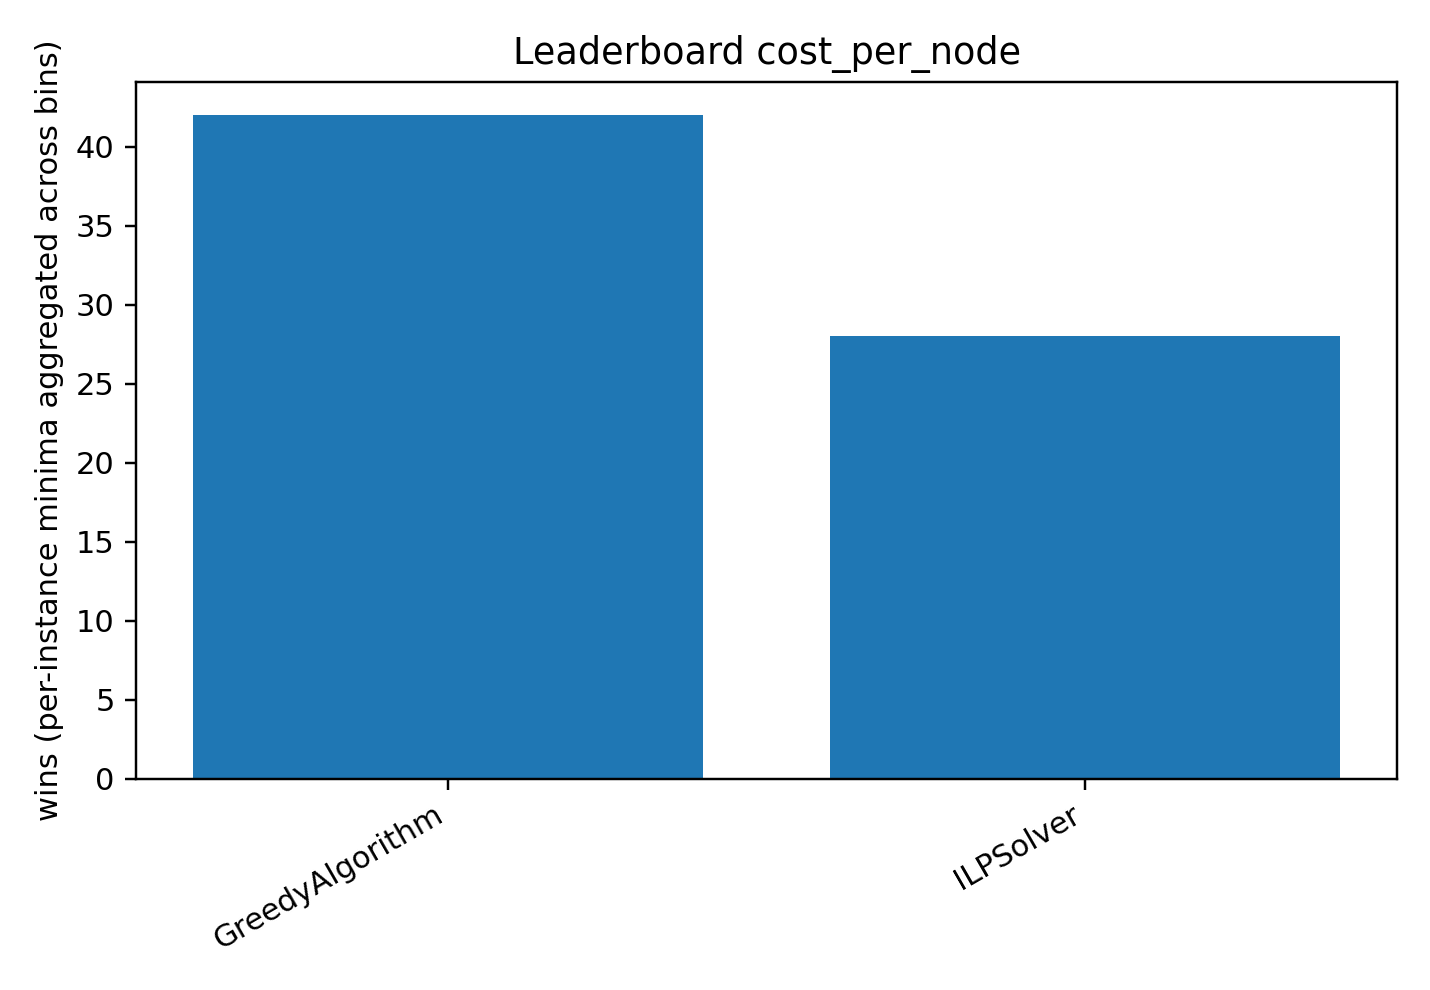
\includegraphics[width=0.48\linewidth]{assets/figures/br_leaderboard_cost.png}
  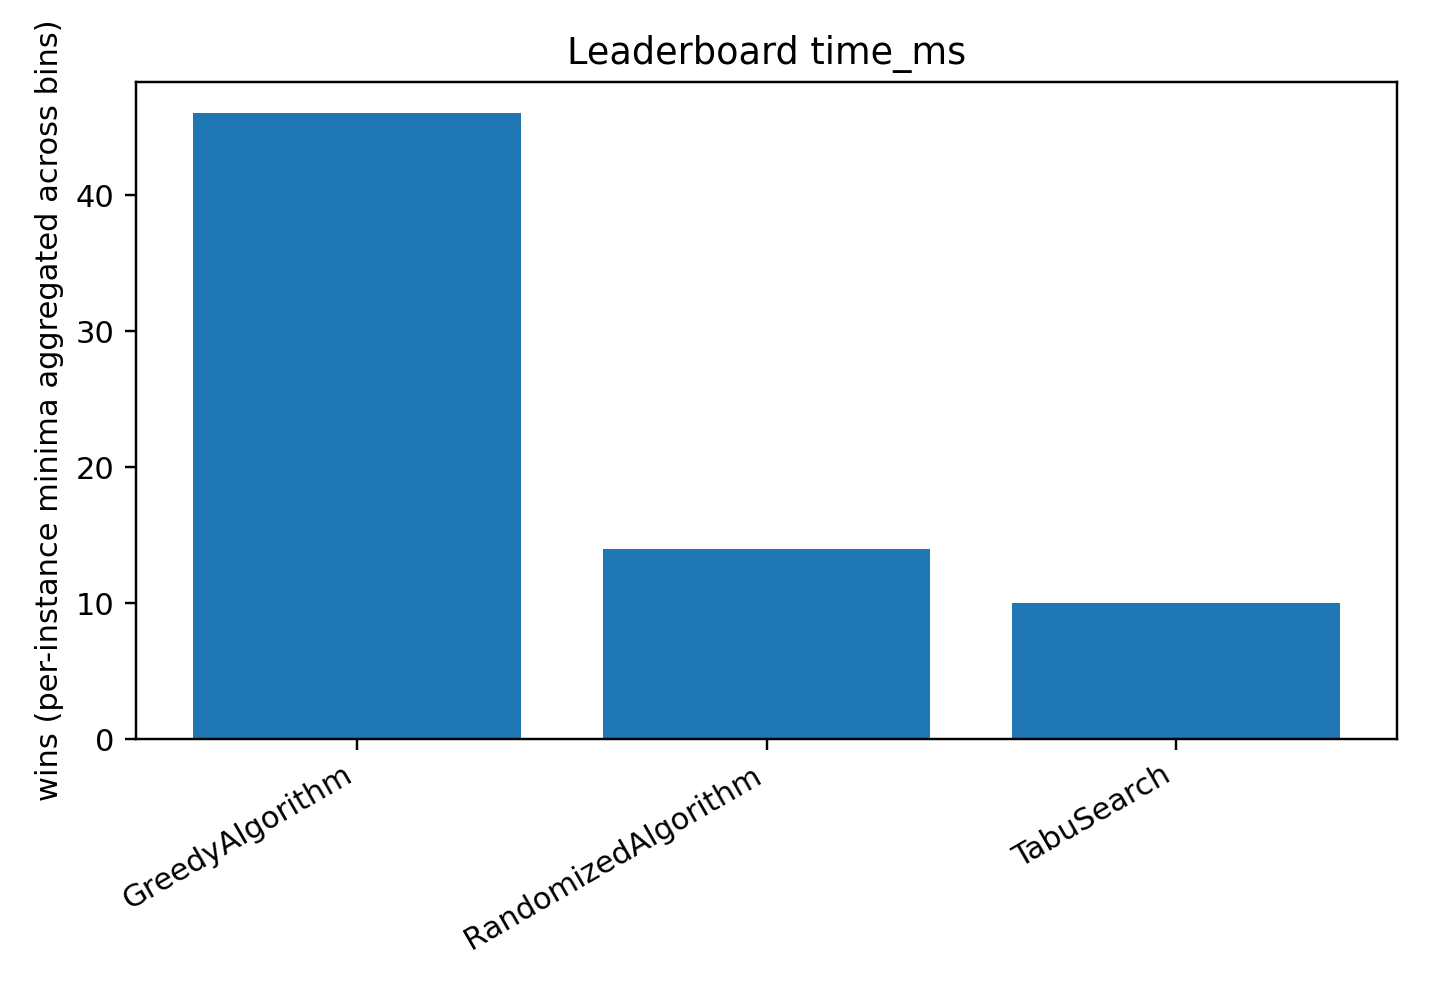
\includegraphics[width=0.48\linewidth]{assets/figures/br_leaderboard_time.png}
  \caption{Porównanie algorytmów na sieciach rzeczywistych (Facebook ego): koszt i czas.}
  \label{fig:facebook_results}
\end{figure}

Na grafach rzeczywistych obserwacje są podobne jak dla grafów syntetycznych. Algorytm zachłanny nadal oferuje najlepszy kompromis, a metaheurystyki dają nieco lepsze wyniki kosztowe za cenę dłuższego czasu obliczeń.

\section{Granice wykonalności ILP}

ILP daje optymalne rozwiązania, ale ma ograniczenia czasowe. Na poniższym wykresie przedstawiono, gdzie solver CBC zaczyna przekraczać limit 60 sekund.

\begin{figure}[h]
  \centering
  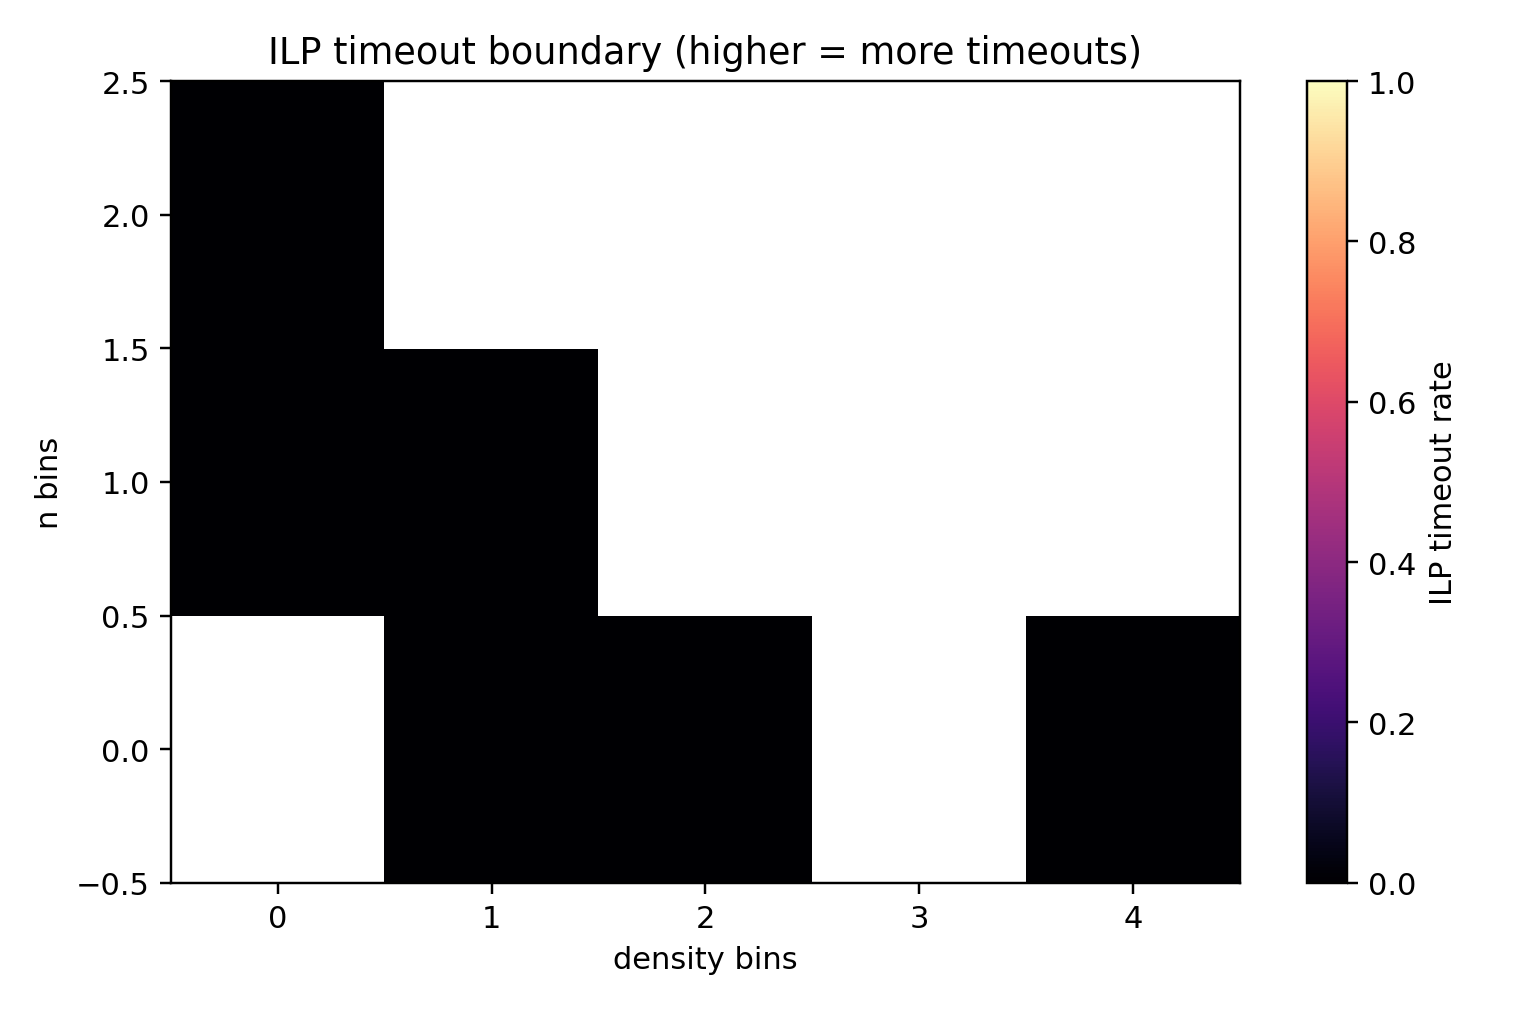
\includegraphics[width=0.7\linewidth]{assets/figures/ba_ilp_timeout_boundary.png}
  \caption{Granice czasowe ILP (solver CBC) w zależności od rozmiaru i gęstości grafu.}
  \label{fig:ilp_limits}
\end{figure}

Widać, że ILP pracuje dobrze do około 100-200 wierzchołków dla grafów o normalnej gęstości. Powyżej tej granicy timeouty stają się częste i potrzebne są heurystyki.

\section{Wnioski}

\paragraph{Najważniejsze obserwacje:}
\begin{itemize}
  \item \textbf{Algorytm zachłanny} jest najlepszym wyborem dla większości praktycznych zastosowań -- szybki i daje dobre wyniki
  \item \textbf{ILP} daje optymalne rozwiązania, ale tylko dla małych grafów (do ~100-200 wierzchołków)
  \item \textbf{Metaheurystyki} warto stosować gdy czas nie jest problemem, a priorytetem jest jak najniższy koszt
  \item \textbf{Struktura grafu} ma kluczowy wpływ -- huby i większa gęstość pozwalają na niższe koszty
  \item \textbf{Konfiguracja duolingo\_super} jest ogólnie bardziej opłacalna niż roman\_domination
\end{itemize}

\paragraph{Rekomendacje praktyczne:}
Dla systemu dystrybucji licencji w sieci znajomych rekomendowany jest algorytm zachłanny jako rozwiązanie domyślne, z opcją przełączenia na metaheurystyki dla najważniejszych klientów gdzie każda oszczędność ma znaczenie.

\paragraph{Analiza kompromisów:}
Fronty Pareto wyraźnie pokazują, że nie ma jednego najlepszego algorytmu -- wybór zależy od priorytetów:
\begin{itemize}
  \item Jeśli czas jest krytyczny -- wybierz greedy
  \item Jeśli koszt jest najważniejszy -- użyj metaheurystyk
  \item Dla małych sieci (<200 węzłów) -- ILP da optimum
  \item Dla dużych sieci -- metaheurystyki z warm startem z greedy
\end{itemize}
